% ============================================================
% Capítulo 02: Arquitetura Antes do Código
% ============================================================
\chapter{Arquitetura Antes do Código}

\section{Introdução}

O maior mito da engenharia de software contemporânea é a ideia de que se deve
``começar a codar e ir ajustando pelo caminho''. Essa mentalidade, frequentemente
confundida com agilidade, é na verdade o oposto do que os manifesto ágil propõe.
Ajustes são necessários, sim, porque toda arquitetura evolui com o tempo. Porém,
começar sem direção, sem um modelo mental do sistema, sem entender as forças que
atuam sobre ele, é o que podemos chamar de \textbf{falsa agilidade}: a ilusão
de velocidade que se paga com retrabalho exponencial.

Para entender por que esse mito é tão perigoso, considere o que acontece quando
uma equipe de cinco engenheiros começa a construir um sistema de pagamentos sem
nenhuma discussão arquitetural prévia. Nas primeiras duas semanas, tudo parece
fluir: cada pessoa escolhe suas ferramentas favoritas, cria endpoints, conecta
ao banco de dados, e o sistema ``funciona'' em demonstrações. Mas por
volta da sexta semana, os problemas começam a emergir. Um engenheiro modelou o
conceito de ``transação'' de uma forma, outro modelou de forma completamente
diferente. As chamadas entre módulos formaram uma teia de dependências circulares.
A performance degrada porque três partes do sistema fazem consultas redundantes
ao banco. E o pior: corrigir qualquer um desses problemas agora exige reescrever
código que já está em produção, com clientes reais usando. O custo de não pensar
a arquitetura antes não é pago no início. É pago depois, com juros compostos.

Ágil não significa sem arquitetura. Significa arquitetura \textbf{evolutiva},
não ausente. Os métodos ágeis reconhecem que não se pode prever tudo no início,
mas isso não é licença para ignorar o pensamento arquitetural. Pelo contrário:
é justamente porque o futuro é incerto que precisamos de estruturas que acomodem
mudança. Pular a fase de arquitetura é como construir um prédio sem planta;
ele pode até ficar de pé, mas vai custar dez vezes mais para consertar quando
os problemas inevitavelmente aparecerem. O próprio Kent Beck, um dos signatários
originais do Manifesto Ágil, nunca advogou pela ausência de design. O que ele
propôs foi design incremental, onde decisões são tomadas no momento mais
responsável: nem cedo demais (quando falta informação), nem tarde demais
(quando o custo de mudança já explodiu).

O papel do pensamento arquitetural é tomar decisões \textbf{antes} que elas se
tornem irreversíveis. Quando você escolhe um banco de dados, um protocolo de
comunicação entre serviços, ou uma estratégia de deploy, está definindo restrições
que serão caras para mudar depois. Essas são as decisões que merecem reflexão
antecipada. Não se trata de criar um documento de 200 páginas que ninguém vai
ler. Trata-se de pensar, discutir e registrar as escolhas que importam. Martin
Fowler chama essas de ``decisões que são difíceis de reverter'', e essa
irreversibilidade justifica o investimento de tempo em reflexão
arquitetural. Escolher a cor de um botão é facilmente reversível; escolher que
o sistema inteiro será baseado em microsserviços comunicando via gRPC não é.

Este capítulo conecta-se diretamente com o que discutimos no Capítulo~1: o
RM-ODP nos dá a estrutura para olhar um sistema sob múltiplos pontos de vista.
Agora, vamos aplicar essa visão explorando estilos arquiteturais,
técnicas de modelagem de domínio, registros de decisão e padrões de migração.
Vamos sair do abstrato e entrar no concreto, com diagramas, código e estudos
de caso. Cada conceito que apresentaremos aqui não existe isoladamente; ele
se conecta com os demais como peças de um quebra-cabeça, e ao final do capítulo,
você terá uma visão integrada de como essas peças se encaixam.

Como vimos no Capítulo~0, o pensamento sistêmico é o que diferencia o engenheiro
do programador. Neste capítulo, esse pensamento se materializa em escolhas
arquiteturais que definem o destino de um projeto. Dominar arquitetura não é
conhecer todos os padrões, e sim saber escolher o padrão certo para o contexto
certo, e explicar o porquê. E, talvez mais importante, é saber quando
\textit{não} escolher um padrão sofisticado, quando a simplicidade é a melhor
arquitetura possível.


\section{Princípios de Design Arquitetural}

Antes de mergulhar nos estilos e padrões, precisamos estabelecer os princípios
fundamentais que guiam qualquer decisão arquitetural. Esses princípios não são
regras rígidas; são heurísticas que orientam o julgamento do engenheiro em
situações de incerteza. Eles existem há décadas, alguns desde os primórdios da
ciência da computação, e continuam relevantes porque atacam problemas
fundamentais da complexidade de software, problemas que não mudam com a
tecnologia da moda.

Pense nesses princípios como as leis da física para o engenheiro de software.
Um engenheiro civil não precisa recitar as leis de Newton a cada viga que calcula,
mas sua intuição sobre estruturas foi moldada por essas leis durante anos de
estudo. Da mesma forma, os princípios que veremos a seguir devem se tornar parte
da intuição do engenheiro de software, guiando suas decisões mesmo quando ele
não está conscientemente ``aplicando um princípio''.

\subsection{Separação de Responsabilidades (SoC)}

O princípio de separação de responsabilidades (Separation of Concerns) afirma
que cada parte do sistema deve cuidar de exatamente uma preocupação. O módulo
que gerencia autenticação não deve saber como funciona a persistência de dados.
O componente que renderiza a interface do usuário não deve conter lógica de
negócio. Quando essas fronteiras são respeitadas, o sistema se torna mais fácil
de entender, testar e modificar.

Edsger Dijkstra articulou essa ideia pela primeira vez em 1974, em um
artigo seminal onde argumentou que a única forma de lidar com a complexidade
de programas grandes é dividi-los em partes que possam ser compreendidas
independentemente. Dijkstra não estava falando de uma técnica de programação,
mas de uma limitação cognitiva humana. O cérebro humano consegue
manter entre cinco e nove coisas na memória de trabalho ao mesmo tempo. Se um
módulo exige que o programador pense simultaneamente em autenticação, formatação
de dados, regras de negócio e comunicação com banco de dados, esse programador
está operando além de sua capacidade cognitiva, e erros são inevitáveis.

SoC se manifesta em múltiplos níveis. No nível de código, significa
funções e classes com responsabilidades claras. Uma função que calcula o imposto
sobre uma transação não deve também formatar o resultado para exibição na tela.
No nível de módulos, significa fronteiras bem definidas entre subsistemas. O
módulo de pagamentos não deve conter código de geração de relatórios, mesmo que
ambos usem dados de transações. No nível de sistema, significa separação entre
camadas (apresentação, lógica de negócio, acesso a dados) ou entre contextos de
domínio. Cada nível de separação reduz a carga cognitiva de quem trabalha no
sistema e aumenta a capacidade de mudança independente.

Um sinal claro de que SoC está sendo violado é quando uma mudança em uma parte
do sistema exige alterações em partes aparentemente não relacionadas. Se mudar o
formato de uma data na interface do usuário requer alterações no módulo de
persistência, algo está fundamentalmente errado com a separação de
responsabilidades.

\subsection{Coesão e Acoplamento}

Coesão e acoplamento são as duas faces da mesma moeda. \textbf{Coesão} mede
o grau em que os elementos dentro de um módulo pertencem juntos. Se uma classe
faz cinco coisas não relacionadas, sua coesão é baixa e ela deveria ser dividida.
\textbf{Acoplamento} mede o grau em que módulos dependem uns dos outros. Se o
módulo A precisa conhecer detalhes internos do módulo B para funcionar, o
acoplamento entre eles é alto, e qualquer mudança em B potencialmente quebra A.

Esses conceitos foram formalizados por Larry Constantine e Edward Yourdon no
final dos anos 1970, no contexto do design estruturado. Quase cinquenta anos
depois, eles permanecem como os indicadores mais confiáveis da qualidade de um
design de software. Não é por acaso: coesão e acoplamento capturam algo
fundamental sobre como humanos entendem e modificam sistemas complexos. Um módulo
coeso é compreensível porque tudo dentro dele ``faz sentido junto'', sem
surpresas, sem funcionalidades escondidas. Um módulo com baixo acoplamento é
modificável porque suas dependências são poucas e bem definidas. Mudar algo
dentro dele não causa efeitos cascata imprevisíveis.

Busca-se maximizar coesão (elementos relacionados juntos) e minimizar
acoplamento (módulos independentes entre si). Isso não é uma busca por perfeição,
é uma heurística pragmática. Algum acoplamento é inevitável; o que importa
é torná-lo explícito e controlado, preferencialmente através de interfaces
estáveis. Um sistema com zero acoplamento seria um conjunto de programas
independentes que não fazem nada juntos. O ponto ideal é ter acoplamento onde
ele é necessário (módulos que realmente precisam colaborar) e evitá-lo onde ele
é acidental (módulos que se acoplaram por conveniência, não por necessidade).

Para ilustrar a diferença entre acoplamento necessário e acidental, considere um
sistema de e-commerce. O módulo de carrinho de compras \textit{precisa} se
comunicar com o módulo de estoque para verificar disponibilidade --- esse é um
acoplamento necessário. Porém, se o módulo de carrinho acessa diretamente as
tabelas do banco de dados do módulo de estoque, em vez de usar uma interface
definida, esse acoplamento de implementação é acidental e perigoso. Qualquer
mudança no schema do banco de estoque vai quebrar o carrinho.

\subsection{Interfaces Estáveis, Implementações Voláteis}

Um dos princípios mais poderosos da engenharia de software é a separação entre
contrato e implementação. A interface de um \texttt{RepositorioDeClientes} define
\textit{o que} pode ser feito (buscar, salvar, atualizar). A implementação define
\textit{como} é feito (SQL, NoSQL, arquivo, API externa). Quando essa separação
é respeitada, a implementação pode ser trocada sem afetar nenhum consumidor da
interface.

Esse princípio tem raízes profundas na história da computação. David Parnas, em
seu artigo de 1972 ``On the Criteria to Be Used in Decomposing Systems into
Modules'', argumentou que módulos devem esconder suas decisões de implementação
atrás de interfaces estáveis. Parnas chamou isso de ``information hiding'',
ocultação de informação. A ideia é que cada módulo esconde uma ``decisão de
design'' que pode mudar no futuro: qual algoritmo de ordenação usar, qual formato
de armazenamento adotar, qual protocolo de comunicação empregar. Se essa decisão
está escondida atrás de uma interface, ela pode ser mudada sem afetar o resto
do sistema.

Esse princípio é a base da arquitetura hexagonal, que discutiremos em detalhes
mais adiante. Ele também está intimamente ligado ao Princípio de Inversão de
Dependência do SOLID: módulos de alto nível não devem depender de módulos de
baixo nível; ambos devem depender de abstrações. Concretamente, isso significa que
a lógica de negócio de um sistema de pagamentos não deve depender diretamente
do PostgreSQL, e sim de uma abstração de ``repositório de transações''
que pode ser implementada com PostgreSQL, MongoDB, ou até mesmo um arquivo CSV
durante os testes.

\subsection{Lei de Demeter}

A Lei de Demeter, também conhecida como ``princípio do menor conhecimento'',
estabelece que um objeto deve falar apenas com seus ``amigos imediatos''. Isso
significa evitar encadeamentos como
\texttt{a.getB().getC().getD().doSomething()}. Cada ponto nessa cadeia é um
acoplamento adicional: se qualquer estrutura intermediária mudar, o código
quebra. A alternativa é expor apenas as operações necessárias, delegando
internamente.

Formulada em 1987 na Northeastern University, durante o
desenvolvimento do Projeto Demeter (daí o nome), apesar de ser chamada de
``lei'', é melhor entendida como uma heurística forte. Sua violação é um dos
``code smells'' mais confiáveis: código que encadeia múltiplas chamadas está,
quase invariavelmente, sabendo demais sobre a estrutura interna de objetos que
não são de sua responsabilidade. Esse conhecimento excessivo cria fragilidade,
e qualquer reestruturação interna desses objetos quebra o código que depende
da cadeia.

Um exemplo concreto: imagine um sistema de recursos humanos onde o código para
calcular o bônus de um funcionário faz
\texttt{funcionario.getDepartamento().getGerente().getOrcamento().getDisponivel()}.
Esse código sabe que funcionários pertencem a departamentos, que departamentos
têm gerentes, que gerentes têm orçamentos, e que orçamentos têm valores
disponíveis. Se amanhã a estrutura organizacional mudar (por exemplo, gerentes
passam a ser responsáveis por múltiplos departamentos), todo esse código quebra.
A alternativa seria \texttt{funcionario.getOrcamentoDisponivelParaBonus()},
delegando a navegação interna para o próprio objeto que conhece sua estrutura.

Com esses princípios fundamentais estabelecidos, estamos prontos para explorar
como eles se manifestam em estilos arquiteturais concretos. Os princípios são a
bússola; os estilos arquiteturais são os mapas que nos guiam por territórios
específicos.


\section{Estilos Arquiteturais: Um Mergulho Profundo}

Cada estilo arquitetural é uma resposta a um conjunto de forças: escala, complexidade
do domínio, tamanho da equipe, requisitos de disponibilidade, restrições de custo.
Não existe estilo ``melhor''; existe o mais adequado para o contexto. A seguir,
exploramos os principais estilos com profundidade, incluindo seus trade-offs reais
e cenários de aplicação.

Antes de mergulhar nos detalhes, uma observação: estilos
arquiteturais não são mutuamente exclusivos. Um sistema real frequentemente
combina elementos de múltiplos estilos. Um monolito modular pode usar comunicação
por eventos internamente. Um sistema de microsserviços pode ter alguns serviços
implementados como funções serverless. O objetivo não é escolher ``um estilo'' e
segui-lo dogmaticamente, mas entender as forças e trade-offs de cada abordagem
para compor a solução mais adequada ao seu contexto.

\subsection{Monolito Modular}

Um sistema implantado como uma única unidade, mas internamente
organizado em módulos bem separados, com fronteiras claras e interfaces definidas
entre eles. É o estilo mais subestimado da indústria. Muitos engenheiros pulam
diretamente para microsserviços por pressão de tendência, quando um monolito
modular resolveria o problema com uma fração da complexidade.

A história do monolito é, na verdade, a história da própria engenharia de software.
Nas primeiras décadas da computação, todo software era monolítico, não por
escolha consciente, mas porque não havia alternativa prática. Os mainframes dos
anos 1960 e 1970 executavam programas como unidades únicas. Com o advento da
computação distribuída nos anos 1980 e 1990, surgiram as primeiras alternativas,
como CORBA e DCOM, mas a complexidade dessas tecnologias era tão grande que
muitos projetos fracassaram espetacularmente. O pêndulo voltou para o monolito
nos anos 2000, com frameworks como Ruby on Rails e Django, que tornaram
extremamente produtivo construir aplicações monolíticas. Então, por volta de
2012--2015, a revolução dos microsserviços, liderada por empresas como Netflix
e Amazon, criou a impressão de que monolitos eram ``legados'' e ``antiquados''.
Essa impressão é incorreta.

O que essas empresas na verdade fizeram foi migrar de monolitos \textit{mal
estruturados} (conhecidos pejorativamente como ``big ball of mud'') para
microsserviços. O problema não era o monolito em si, era a falta de
estrutura interna. Um monolito modular, com fronteiras claras entre
módulos, interfaces estáveis e separação de responsabilidades, oferece
a maioria dos benefícios organizacionais que motivaram a migração para
microsserviços, sem a complexidade operacional distribuída.

As vantagens são significativas. A simplicidade operacional é talvez a maior
delas: há um único artefato para implantar, monitorar e depurar. Quando algo
dá errado às três da manhã, o engenheiro de plantão precisa investigar um
sistema, não vinte. As transações são locais, o que significa que a consistência
de dados é garantida pelo banco de dados relacional, sem a complexidade de
sagas ou compensações que sistemas distribuídos exigem. A refatoração é
facilitada porque tudo está no mesmo processo: ferramentas de IDE como ``Find
All References'' e ``Rename Symbol'' funcionam perfeitamente, coisa que é
praticamente impossível em um ecossistema de microsserviços.

As desvantagens são reais, mas frequentemente exageradas. A escala é ``tudo
ou nada'': o sistema inteiro escala junto, mesmo que apenas um módulo esteja
sob pressão. Há risco de erosão das fronteiras internas com o tempo; sem
disciplina, os módulos se acoplam progressivamente, e o que começou como um
monolito modular degenera em um ``big ball of mud''. Há também um limite prático
de tamanho de equipe: quando dezenas de engenheiros trabalham no mesmo
repositório, os conflitos de merge e a coordenação de releases se tornam
custosos.

O monolito modular é ideal para times pequenos a médios (até 30--40 pessoas),
domínios cuja complexidade ainda está sendo descoberta, e projetos que priorizam
velocidade de entrega sobre escala granular. Empresas como Shopify demonstram
que é possível operar monolitos modulares massivos com sucesso: o monolito
principal da Shopify serve centenas de milhares de lojas online com bilhões
de dólares em transações. A Basecamp, criadora do Ruby on Rails, opera há
mais de vinte anos com uma arquitetura monolítica e uma equipe relativamente
pequena. O Stack Overflow, um dos sites mais acessados do mundo, processou
bilhões de page views com um monolito em C\# e uma equipe de menos de vinte
desenvolvedores.

\subsection{Microsserviços}

A arquitetura de microsserviços decompõe o sistema em serviços independentes, cada
um com seu próprio ciclo de vida, banco de dados e equipe responsável. Cada serviço
é implantado de forma independente e se comunica com os demais via rede (HTTP, gRPC,
mensageria).

O termo ``microsserviços'' foi popularizado por volta de 2011--2012, embora a
ideia de serviços independentes comunicando via rede existisse há muito mais
tempo sob nomes como SOA (Service-Oriented Architecture). A diferença crucial
é que SOA tipicamente envolvia grandes serviços monolíticos comunicando via
ESBs (Enterprise Service Buses) pesados e protocolos como SOAP. Os
microsserviços propuseram serviços menores, mais leves, comunicando via
protocolos simples como HTTP/REST, e com governança descentralizada, onde cada
time é dono de seus serviços e pode tomar decisões tecnológicas independentes.

As vantagens são reais em contextos específicos. A escala seletiva permite
escalar apenas o serviço que está sob pressão: se o serviço de busca recebe
dez vezes mais tráfego que o serviço de cadastro, apenas o serviço de busca
precisa de mais instâncias. A autonomia de times é poderosa em organizações
grandes: cada equipe é dona do seu serviço, pode fazer deploy independente,
pode até escolher linguagens de programação diferentes se isso fizer sentido.
O isolamento de falhas, quando bem implementado, significa que a queda de um
serviço não derruba o sistema inteiro. O catálogo de produtos pode continuar
funcionando mesmo que o sistema de recomendações esteja fora do ar.

Porém, as desvantagens são frequentemente subestimadas, especialmente por
equipes que nunca operaram sistemas distribuídos em produção. A complexidade
distribuída é real e insidiosa: a rede falha, a latência é imprevisível, e
o debugging é exponencialmente mais difícil quando uma requisição percorre
cinco serviços diferentes antes de retornar uma resposta. Há necessidade de
infraestrutura robusta que não existia antes: service discovery para que
serviços encontrem uns aos outros, load balancing distribuído, circuit
breakers para evitar falhas em cascata, tracing distribuído para entender
o caminho de uma requisição, e dashboards de observabilidade que monitorem
dezenas ou centenas de serviços simultaneamente.

A consistência de dados é talvez o desafio mais subestimado. Em um monolito,
uma transação bancária que debita de uma conta e credita outra é uma
transação ACID simples. Em microsserviços, onde cada serviço tem seu próprio
banco, essa mesma operação requer um padrão de saga: uma sequência de
transações locais coordenadas por eventos ou orquestração, com operações de
compensação para cada passo que pode falhar. A complexidade de implementar
sagas corretamente é enorme, e bugs nesse nível causam inconsistências de
dados que são extremamente difíceis de diagnosticar e corrigir.

A história da indústria está repleta de cautionary tales. A própria Amazon,
frequentemente citada como pioneira dos microsserviços, levou anos e centenas
de engenheiros para fazer a transição funcionar. Empresas menores que tentaram
imitar a Amazon sem ter os mesmos recursos frequentemente terminaram com o
pior dos dois mundos: a complexidade dos microsserviços sem os benefícios,
porque seus serviços eram tão acoplados que não podiam ser deployados
independentemente de qualquer forma. O termo ``distributed monolith'' (um
monolito distribuído) foi cunhado para descrever essa situação
infeliz.

A regra de ouro que propomos neste livro é direta: \textbf{comece monolítico e
modular; separe quando a dor justificar}. Nunca separe por antecipação. A dor
que justifica microsserviços é concreta: times que não conseguem mais trabalhar
no mesmo repositório sem conflitos constantes, necessidade comprovada de escalar
partes do sistema independentemente, ou requisitos regulatórios de isolamento.
Se você não está sentindo essa dor, microsserviços vão adicionar complexidade
sem benefício correspondente.

\subsection{Arquitetura Orientada a Eventos}

Na arquitetura orientada a eventos, os componentes se comunicam publicando e
consumindo eventos, em vez de fazer chamadas diretas uns aos outros. Um evento
representa algo que aconteceu: ``PedidoFoiCriado'', ``PagamentoFoiConfirmado'',
``EstoqueFoiReservado''. Componentes interessados reagem a esses eventos de
forma assíncrona.

Sistemas orientados a eventos têm raízes que remontam aos anos 1980,
com os primeiros sistemas de publish-subscribe. O estilo, contudo, ganhou
enorme tração com o advento do Apache Kafka em 2011, criado pela equipe de
engenharia do LinkedIn para lidar com o volume massivo de eventos gerados pela
plataforma. O Kafka transformou a arquitetura orientada a eventos de uma ideia
acadêmica em uma ferramenta prática, ao resolver dois problemas que os sistemas
de mensageria anteriores não resolviam bem: a persistência de eventos (permitindo
replay) e o throughput necessário para escala de internet.

Esse estilo oferece desacoplamento temporal, o que significa que o produtor não
precisa esperar o consumidor processar o evento. Quando o serviço de pedidos
publica ``PedidoCriado'', ele não sabe e não se importa se o serviço de
estoque, o serviço de notificações e o serviço de analytics vão processar esse
evento em milissegundos ou em minutos. Essa independência temporal é libertadora
para a escalabilidade, porque novos consumidores podem ser adicionados sem
alterar o produtor, e consumidores lentos não bloqueiam o produtor.

A resiliência é outro benefício significativo. Se o serviço de notificações está
fora do ar quando um pedido é criado, o evento fica na fila esperando. Quando o
serviço volta, ele processa todos os eventos pendentes. Em uma arquitetura
síncrona (chamadas HTTP diretas), essa mesma situação causaria erros ou
timeouts no serviço de pedidos, afetando a experiência do usuário.

Porém, a arquitetura orientada a eventos traz desafios significativos que não
devem ser subestimados. A consistência eventual é o mais fundamental: quando um
evento é publicado, pode levar tempo até que todos os consumidores o processem.
Durante esse intervalo, partes do sistema têm visões diferentes da realidade. O
serviço de pedidos sabe que o pedido foi criado, mas o serviço de estoque ainda
não reservou os itens. Lidar com essas janelas de inconsistência requer design
cuidadoso e comunicação clara com stakeholders que esperavam consistência
imediata.

O debugging é outro desafio considerável. Rastrear o fluxo de um evento
através de múltiplos consumidores exige ferramentas específicas de
observabilidade, como distributed tracing. Sem essas ferramentas, quando algo
dá errado (um pedido foi criado mas a notificação nunca chegou), é
extremamente difícil determinar onde o evento se perdeu. A ordenação de
eventos adiciona outra camada de complexidade: garantir que eventos sejam
processados na ordem correta é surpreendentemente difícil em sistemas
distribuídos, e processar eventos fora de ordem pode levar a estados
inconsistentes difíceis de diagnosticar.

O diagrama a seguir ilustra uma arquitetura orientada a eventos para um sistema
de pedidos:

\begin{figure}[htbp]
    \centering
    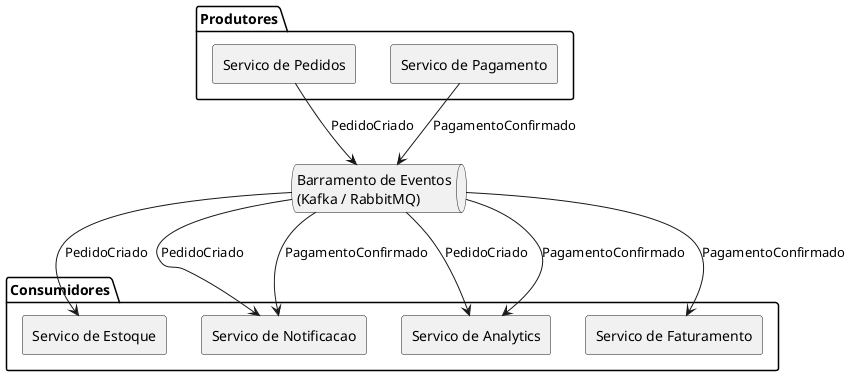
\includegraphics[width=0.85\textwidth]{imagens/02-arquitetura-antes-do-codigo-01-plantuml-arquitetura-orientada-a-eventos.png}
    \caption{PlantUML -- Arquitetura Orientada a Eventos}
\end{figure}

Observe como o serviço de pedidos não sabe (e não precisa saber) quem vai reagir
ao evento \texttt{PedidoCriado}. Amanhã, um novo serviço de recomendação pode
começar a consumir esse evento sem qualquer alteração no produtor. Esse é o poder
do desacoplamento via eventos. E esse poder tem uma implicação organizacional
importante: times podem trabalhar de forma independente, cada um publicando e
consumindo os eventos que lhe interessam, sem precisar coordenar deploys ou
negociar interfaces síncronas. É uma forma de desacoplamento que vai além do
técnico; é desacoplamento organizacional.

\subsection{Serverless}

O modelo serverless leva a abstração ao extremo: o engenheiro escreve funções
individuais que são executadas sob demanda, sem gerenciar servidores, containers
ou infraestrutura. O provedor de nuvem cuida de escala, disponibilidade e
cobrança por uso efetivo.

A história do serverless começa em 2014, quando a Amazon lançou o AWS Lambda.
A promessa era sedutora: escreva apenas a lógica de negócio, e a infraestrutura
``desaparece''. Não há servidores para provisionar, não há sistemas operacionais
para atualizar, não há containers para orquestrar. Você paga apenas pelo tempo
de execução das suas funções, medido em milissegundos. Para workloads com
tráfego esporádico, isso pode significar uma redução de custos de 90\% ou mais
em relação a servidores tradicionais que ficam rodando 24 horas por dia
esperando requisições.

As vantagens são genuinamente atraentes. O custo proporcional ao uso significa
que uma startup pré-receita pode operar com custos de infraestrutura
praticamente zero durante o desenvolvimento, pagando apenas quando usuários
reais começam a usar o sistema. O zero de operação de infraestrutura libera
engenheiros que seriam dedicados a DevOps para trabalhar em funcionalidades de
produto. E a escala automática é impressionante: uma função Lambda pode ir de
zero a milhares de instâncias simultâneas em segundos, sem qualquer configuração
de autoscaling.

As desvantagens, porém, são estruturais e não devem ser minimizadas. Os cold
starts (a latência adicional na primeira invocação, quando o ambiente de
execução da função precisa ser inicializado) são problemáticos para
aplicações que exigem respostas rápidas e consistentes. Dependendo da
linguagem e do tamanho do pacote, um cold start pode adicionar de 100ms a
vários segundos de latência. O vendor lock-in é severo: cada provedor de
nuvem tem suas próprias APIs, limites e peculiaridades. Uma função Lambda
escrita para AWS não roda no Azure Functions sem reescrita significativa.
Os limites de execução são reais: tempo máximo de execução (15 minutos no
Lambda), memória limitada, tamanho de payload restrito. E testar localmente
é notoriamente difícil, porque o ambiente de execução do provedor de nuvem
tem características que não são facilmente reproduzidas em uma máquina de
desenvolvimento.

Serverless brilha em cenários de processamento de eventos (webhooks,
transformação de dados, pipelines ETL), APIs com tráfego altamente variável
onde os picos são esporádicos e imprevisíveis, e automações internas que
rodam periodicamente (cron jobs). Empresas como a iRobot usam Lambda
extensivamente para processar eventos de milhões de robôs aspiradores
conectados. A Coca-Cola utilizou serverless para construir máquinas de venda
conectadas, onde o tráfego é extremamente esporádico mas precisa ser processado
rapidamente quando ocorre.

Serverless não é adequado para workloads de longa duração que excedem os
limites de tempo de execução, sistemas com requisitos de latência rigorosos
onde cold starts são inaceitáveis, ou domínios complexos onde a lógica de
negócio precisa de estado conversacional mantido entre invocações. Também não
é ideal quando a previsibilidade de custos é importante: embora serverless
seja barato para cargas baixas, o custo pode escalar rapidamente com o
volume, e funções mal otimizadas podem gerar faturas surpreendentes.

\subsection{Tabela Comparativa de Estilos Arquiteturais}

Cada estilo arquitetural carrega consigo um conjunto de trade-offs que precisa
ser avaliado no contexto específico do projeto em questão. Não existe almoço
grátis em arquitetura de software: cada vantagem é contrabalanceada por um
custo, e a arte do engenheiro está em escolher os trade-offs que são aceitáveis
para sua situação. A tabela a seguir sintetiza os trade-offs de cada estilo
para facilitar a decisão:

\begin{table}[htbp]
\centering
\caption{Quando usar cada estilo arquitetural}
\label{tab:estilos-arquiteturais}
\small
\begin{tabular}{p{2.8cm}p{2.5cm}p{2.5cm}p{2.5cm}p{2.5cm}}
\toprule
\textbf{Critério} & \textbf{Monolito Modular} & \textbf{Microsserviços} & \textbf{Event-Driven} & \textbf{Serverless} \\
\midrule
Complexidade operacional & Baixa & Alta & Média--Alta & Baixa \\
\addlinespace
Escala & Uniforme & Granular & Granular & Automática \\
\addlinespace
Tamanho de time ideal & 3--40 pessoas & 40+ pessoas & Variável & 3--15 pessoas \\
\addlinespace
Consistência de dados & Forte (ACID) & Eventual & Eventual & Eventual \\
\addlinespace
Debugging & Simples & Complexo & Complexo & Moderado \\
\addlinespace
Custo inicial & Baixo & Alto & Médio & Baixo \\
\addlinespace
Custo de mudança & Médio & Alto & Médio & Baixo \\
\addlinespace
Vendor lock-in & Nenhum & Baixo & Baixo--Médio & Alto \\
\bottomrule
\end{tabular}
\end{table}

Esta tabela é uma simplificação deliberada. Cada célula
poderia ser expandida em uma discussão de vários parágrafos. Por exemplo,
``complexidade operacional baixa'' para monolitos é verdade em comparação com
microsserviços, mas isso não significa que operar um monolito grande seja
trivial. Da mesma forma, ``vendor lock-in alto'' para serverless é verdade para
a lógica de orquestração e configuração, mas a lógica de negócio pura dentro
das funções pode ser portável se bem arquitetada. Use a tabela como ponto de
partida para a reflexão, não como resposta definitiva.

\subsection{Evolução: Do Monolito aos Microsserviços}

A evolução arquitetural não é um salto, mas uma jornada. Nenhum sistema nasce
como um ecossistema de microsserviços; todos começam como algo mais simples. A
questão não é ``devo usar microsserviços?'' mas sim ``quando, se algum dia, a
transição se justifica?'' O diagrama a seguir ilustra os estágios típicos que
um sistema percorre, cada transição motivada por dor concreta:

\begin{figure}[htbp]
    \centering
    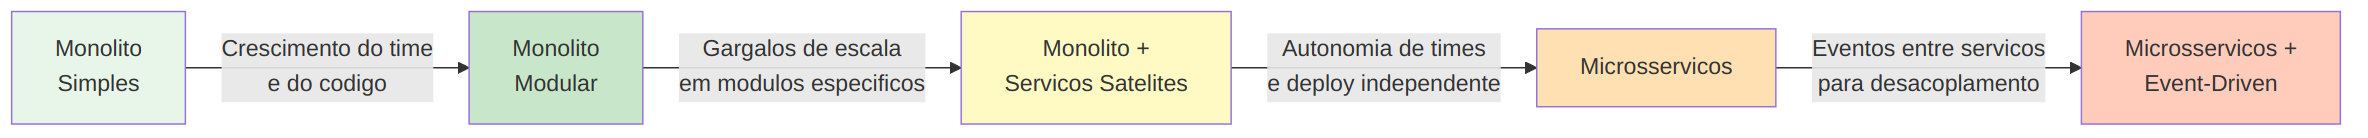
\includegraphics[width=0.85\textwidth]{imagens/02-arquitetura-antes-do-codigo-02-mermaid-evolucao-do-monolito-aos-microsservicos.png}
    \caption{Mermaid -- Evolução do Monolito aos Microsserviços}
\end{figure}

Observe que cada transição tem um gatilho claro. Não se move para o próximo
estágio por moda tecnológica, mas por necessidade comprovada. Muitas empresas
de sucesso operam confortavelmente no estágio de monolito modular por anos.
Outras precisam chegar ao estágio de event-driven para atender a demandas de
escala e resiliência. O importante é que cada decisão de transição seja consciente
e documentada (veremos como fazer isso com ADRs adiante).

A história da indústria oferece lições valiosas sobre essa jornada. O Twitter
começou como um monolito em Ruby on Rails. Quando o tráfego explodiu após
eventos como a Copa do Mundo e eleições americanas, a equipe precisou migrar
para uma arquitetura de serviços, um processo doloroso que levou anos e
envolveu reescritas em Scala e Java. O Spotify seguiu um caminho semelhante,
mas com mais planejamento: começou monolítico, modularizou, e depois extraiu
serviços gradualmente, cada extração motivada por uma necessidade concreta de
escala ou autonomia de time. O importante em ambos os casos é que a migração
foi motivada por dor real, não por tendência tecnológica.

A transição entre estilos arquiteturais nos leva naturalmente a uma pergunta
fundamental: como comunicamos a arquitetura que escolhemos? Como garantimos que
todos no time, dos desenvolvedores juniores aos stakeholders executivos,
entendam o que estamos construindo e por quê? É exatamente isso que o modelo C4
se propõe a resolver.


\section{O Modelo C4: Comunicando Arquitetura em Níveis}

Um dos maiores desafios da arquitetura de software não é a decisão técnica em
si, mas a \textbf{comunicação} dessa decisão. Diagramas de arquitetura
frequentemente falham porque tentam mostrar tudo de uma vez, resultando em
artefatos incompreensíveis que ninguém consulta. Quem nunca viu aquele diagrama
Visio com 200 caixas e 500 setas, impresso em tamanho A0 e colado na parede do
escritório, que ninguém entende e que ficou desatualizado três semanas após sua
criação?

O modelo C4, criado por Simon Brown por volta de 2006, resolve esse problema ao
organizar a documentação arquitetural em quatro níveis de zoom, cada um destinado
a uma audiência diferente. O nome ``C4'' vem dos quatro níveis: Context,
Containers, Components e Code. A analogia que Brown usa é a do Google Maps:
quando você abre o aplicativo, vê primeiro o mundo inteiro. Ao dar zoom, vê
países, depois cidades, depois ruas, depois prédios individuais. Ninguém
reclama que o mapa-múndi não mostra as ruas de São Paulo, pois cada nível de
zoom tem seu propósito e sua audiência.

Antes do C4, a documentação arquitetural era dominada pelo UML (Unified Modeling
Language), que oferecia dezenas de tipos de diagramas com notações complexas.
O problema do UML não era a formalidade em si, mas a barreira de entrada: para
ler um diagrama UML, era preciso entender a notação, e para desenhá-lo, era
preciso usar ferramentas especializadas. O resultado prático é que a maioria
dos times simplesmente não documentava sua arquitetura, ou o fazia com
diagramas informais em quadros brancos que se perdiam ao final da reunião. O
C4 propõe um meio-termo: estrutura suficiente para ser útil, simplicidade
suficiente para ser adotado.

\subsection{Nível 1: Contexto do Sistema}

O diagrama de contexto é o nível mais alto. Ele mostra o sistema como uma caixa
preta e mapeia suas relações com usuários e sistemas externos. É o diagrama que
você mostra para stakeholders não técnicos, gerentes de produto e executivos.
A pergunta que ele responde é: ``O que estamos construindo e com quem/o que
ele interage?''

Esse nível é deliberadamente simples. O sistema inteiro é representado por uma
única caixa no centro do diagrama. Ao redor, ficam as ``personas'' (tipos de
usuários que interagem com o sistema) e os ``sistemas externos'' (outras
aplicações, APIs de terceiros, serviços de infraestrutura). As setas indicam
as relações: ``o cliente usa o sistema para fazer pedidos'', ``o sistema envia
e-mails via SendGrid'', ``o sistema consulta taxas de câmbio via API do Banco
Central''.

A regra de ouro para o diagrama de contexto é que qualquer pessoa na organização,
do estagiário ao CEO, deve conseguir entendê-lo em menos de um minuto.
Se o diagrama requer explicação, ele está complexo demais para este nível.
Detalhes técnicos como tecnologias, protocolos e bancos de dados não aparecem
aqui. O foco é exclusivamente nas relações de negócio.

\begin{figure}[htbp]
    \centering
    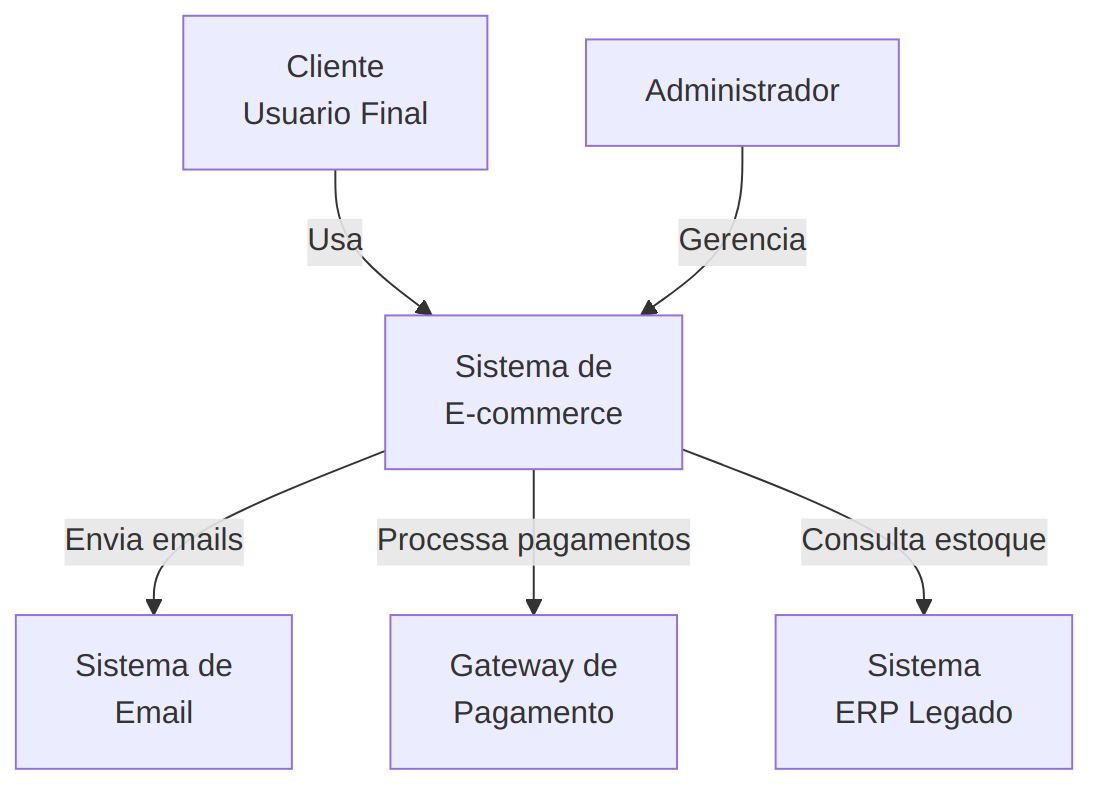
\includegraphics[width=0.85\textwidth]{imagens/02-arquitetura-antes-do-codigo-03-diagrama-c4-nivel-1-contexto-do-sistema.png}
    \caption{Diagrama C4 Nível 1 -- Contexto do Sistema}
\end{figure}

Neste exemplo, vemos imediatamente que o sistema de e-commerce tem dois tipos de
usuários (clientes finais e administradores) e depende de três sistemas externos
(email, pagamento e ERP). Essa simplicidade é intencional, e qualquer pessoa na
organização deve conseguir entender esse diagrama em menos de um minuto. Não há
detalhes técnicos, não há tecnologias mencionadas. Apenas relações de negócio.

\subsection{Nível 2: Containers}

O nível de containers mostra os ``blocos de deployment'' do sistema: aplicações
web, APIs, bancos de dados, filas de mensagens. Cada container é uma unidade que
roda em seu próprio processo ou ambiente. Este é o diagrama que a equipe de
infraestrutura precisa para planejar deployment e monitoramento.

Aqui, ``container'' não se refere a Docker containers,
embora frequentemente coincidam. Um container no modelo C4 é qualquer unidade
de execução separada: uma aplicação web frontend (rodando no browser do
usuário), uma API backend (rodando em um servidor ou container Docker), um
banco de dados (rodando em um servidor dedicado ou serviço gerenciado), uma
fila de mensagens (RabbitMQ, Kafka), um worker de processamento assíncrono.
A pergunta que este nível responde é: ``Quais são as peças que precisamos
rodar e como elas se comunicam?''

Neste nível, tecnologias começam a aparecer. As caixas são rotuladas com a
tecnologia usada: ``API REST em Python/FastAPI'', ``SPA em React'', ``Banco
de dados PostgreSQL'', ``Fila Kafka''. As setas indicam protocolos de
comunicação: ``HTTPS/REST'', ``TCP/gRPC'', ``AMQP''. Esse nível é
particularmente útil para conversas sobre infraestrutura, segurança (quais
containers estão expostos à internet?) e performance (quais comunicações
são síncronas versus assíncronas?).

\subsection{Nível 3: Componentes}

Dentro de cada container, o diagrama de componentes mostra as principais peças
internas: controllers, serviços, repositórios. É o nível que interessa aos
desenvolvedores do time para entender a estrutura interna de um serviço ou
aplicação.

Se o nível de containers mostra ``a API backend'' como uma caixa, o nível de
componentes abre essa caixa e revela o que há dentro. Aqui encontramos os
controllers que recebem requisições HTTP, os serviços de domínio que
implementam a lógica de negócio, os repositórios que acessam o banco de
dados, os publishers que enviam eventos. É neste nível que padrões como
arquitetura hexagonal e separação em camadas se tornam visíveis.

A audiência deste nível é exclusivamente técnica: os desenvolvedores que
vão trabalhar dentro daquele container. Um desenvolvedor que acaba de
entrar no time pode usar o diagrama de componentes para entender rapidamente
a estrutura do código antes de abrir a IDE. Onde ficam as regras de negócio?
Quais são os pontos de entrada? Como os dados fluem do controller até o
banco de dados? Essas perguntas são respondidas visualmente neste nível.

\subsection{Nível 4: Código}

O último nível é o diagrama de classes ou entidades, representando o código em
si. Esse nível raramente é mantido manualmente, pois pode ser
gerado automaticamente a partir do código-fonte. Use-o apenas para partes
críticas do domínio que precisam de documentação explícita.

Simon Brown é enfático sobre este ponto: o nível de código só vale o esforço
de manutenção se estiver representando algo que não é óbvio a partir do
código em si. Para a maioria dos sistemas, o código é sua própria melhor
documentação neste nível de detalhe. A exceção são modelos de domínio
complexos, onde um diagrama de entidades e suas relações pode ajudar
novos membros do time a entender a estrutura antes de mergulhar no código.

A beleza do C4 está na sua disciplina de zoom. Quando alguém pergunta ``como
funciona o sistema?'', você não mostra um diagrama com 200 caixas. Você começa
pelo contexto, e aprofunda sob demanda. Cada nível é autocontido e compreensível
por si só. Essa disciplina de comunicação é uma habilidade arquitetural tão
importante quanto a decisão técnica em si. Um arquiteto que não consegue
comunicar suas decisões de forma clara para audiências diferentes é apenas
alguém que sabe muitas coisas mas não consegue transmiti-las. E conhecimento
não transmitido é conhecimento perdido.

Dominar a comunicação arquitetural por meio do C4 prepara o engenheiro para o
próximo passo: entender o domínio de negócio que a arquitetura
serve. É aqui que entra o Domain-Driven Design, uma abordagem que coloca o
negócio no centro de todas as decisões técnicas.


\section{Modelando com Domínio (DDD)}

Domain-Driven Design, popularizado por Eric Evans em seu livro seminal de 2003
(conhecido carinhosamente como ``The Blue Book'' na comunidade), é uma abordagem
de design de software que coloca o \textbf{domínio do negócio} no centro de todas
as decisões técnicas. Não é um framework, não é uma biblioteca. É uma filosofia
de design que reconhece que a complexidade de um software está na lógica de
negócio, não na tecnologia.

Evans não inventou todas as ideias do DDD do zero. Ele sintetizou décadas de
experiência em projetos de software empresarial, reunindo conceitos que
engenheiros experientes já praticavam intuitivamente, mas que nunca haviam
sido articulados de forma coerente. O mérito de Evans foi dar nomes a esses
conceitos, organizá-los em um framework conceitual, e demonstrar, com
exemplos detalhados de projetos reais, como eles se conectam.

A premissa do DDD é que o maior risco em projetos de software não
é técnico: é a falta de entendimento do domínio. Um sistema tecnicamente
brilhante que modela o domínio de forma errada é inútil. Um sistema
tecnicamente mediano que modela o domínio corretamente pode ser valioso por
décadas. Quantos projetos fracassaram não por falha de banco de dados ou
problemas de performance, mas porque o software simplesmente não fazia o que
o negócio precisava? O DDD ataca esse problema na raiz.

\subsection{Linguagem Ubíqua}

O primeiro e mais importante conceito do DDD é a linguagem ubíqua: engenheiros
e especialistas de negócio devem usar exatamente os mesmos termos. Se o negócio
fala ``sinistro'', o código diz \texttt{Sinistro}, não \texttt{InsuranceClaim}.
Se o negócio fala ``apólice'', o código diz \texttt{Apolice}, não
\texttt{PolicyDocument}. Se o negócio diz ``indenizar'', o método se chama
\texttt{indenizar()}, não \texttt{process()} ou \texttt{handle()}.

Essa prática parece simples, quase trivial, mas sua importância é enorme.
Ela elimina uma das maiores fontes de bugs em software: a tradução mental
entre terminologias. Quando o analista de negócios diz ``o sinistro deve
ser indenizado'' e o programador implementa como \texttt{claim.approve()},
existe uma lacuna semântica que vai gerar mal-entendidos. O analista pode
dizer ``indenizar'' pensando em um processo que inclui verificação de
cobertura, cálculo do valor, e emissão do pagamento. O programador pode
implementar \texttt{approve()} como uma simples mudança de status. A lacuna
entre as duas interpretações é onde os bugs de negócio se escondem, bugs
que passam em todos os testes unitários porque o código faz exatamente o que
foi programado para fazer, mas não faz o que o negócio espera.

Se ambos dizem ``indenizar o sinistro'' e o código diz
\texttt{sinistro.indenizar()}, a comunicação é direta e verificável.
O especialista de domínio pode ler o nome do método e confirmar: ``Sim, isso
é o que queremos dizer com indenizar.'' Essa verificabilidade é impossível
quando os termos do código divergem dos termos do negócio.

A linguagem ubíqua não se limita ao código. Ela deve permear toda a
comunicação do projeto: documentação, tickets no Jira, conversas no Slack,
apresentações para stakeholders. Quando alguém introduz um termo novo ou usa
um sinônimo diferente, isso deve ser discutido e resolvido. É um investimento
de disciplina que paga dividendos enormes ao longo da vida do projeto.

\subsection{Bounded Contexts}

O conceito de bounded context é talvez a contribuição mais transformadora do
DDD para a arquitetura de software. Ele reconhece uma verdade que muitos
engenheiros resistem em aceitar: o mesmo termo pode ter significados
diferentes em contextos diferentes. ``Cliente'' no contexto de Vendas tem
nome, email e histórico de compras. ``Cliente'' no contexto de Suporte tem
tickets abertos, SLA e canal de contato preferido. ``Cliente'' no contexto
Financeiro tem CPF, limite de crédito e inadimplência.

Para entender por que isso importa, imagine um hospital. A palavra ``paciente''
aparece em dezenas de contextos diferentes. Na emergência, um paciente tem
sintomas, triagem e prioridade de atendimento. Na farmácia, um paciente tem
alergias, medicamentos prescritos e interações medicamentosas. Na
contabilidade, um paciente tem convênio, co-participação e faturas. Na UTI,
um paciente tem sinais vitais, medicações contínuas e escala de Glasgow.
Tentar criar um modelo único de ``Paciente'' que sirva para todos esses
contextos é um erro que leva a classes com centenas de campos, a maioria dos
quais é irrelevante para qualquer contexto específico. O resultado é código
confuso, frágil e impossível de evoluir independentemente.

Tentar criar um modelo único de ``Cliente'' que sirva para todos os contextos é
um erro clássico que leva a classes gigantes com dezenas de campos opcionais.
Esse padrão é tão comum que tem um nome informal na comunidade: o ``God Object'',
um objeto que sabe tudo sobre tudo e que precisa mudar toda vez que qualquer
parte do sistema muda. A abordagem do DDD é aceitar que cada contexto tem seu
próprio modelo de Cliente, e definir mapeamentos explícitos entre eles. Quando
o contexto de Vendas precisa informar o contexto Financeiro sobre uma nova venda,
ele publica um evento com apenas as informações necessárias, não o objeto
completo.

O diagrama a seguir ilustra os bounded contexts de um sistema de e-commerce:

\begin{figure}[htbp]
    \centering
    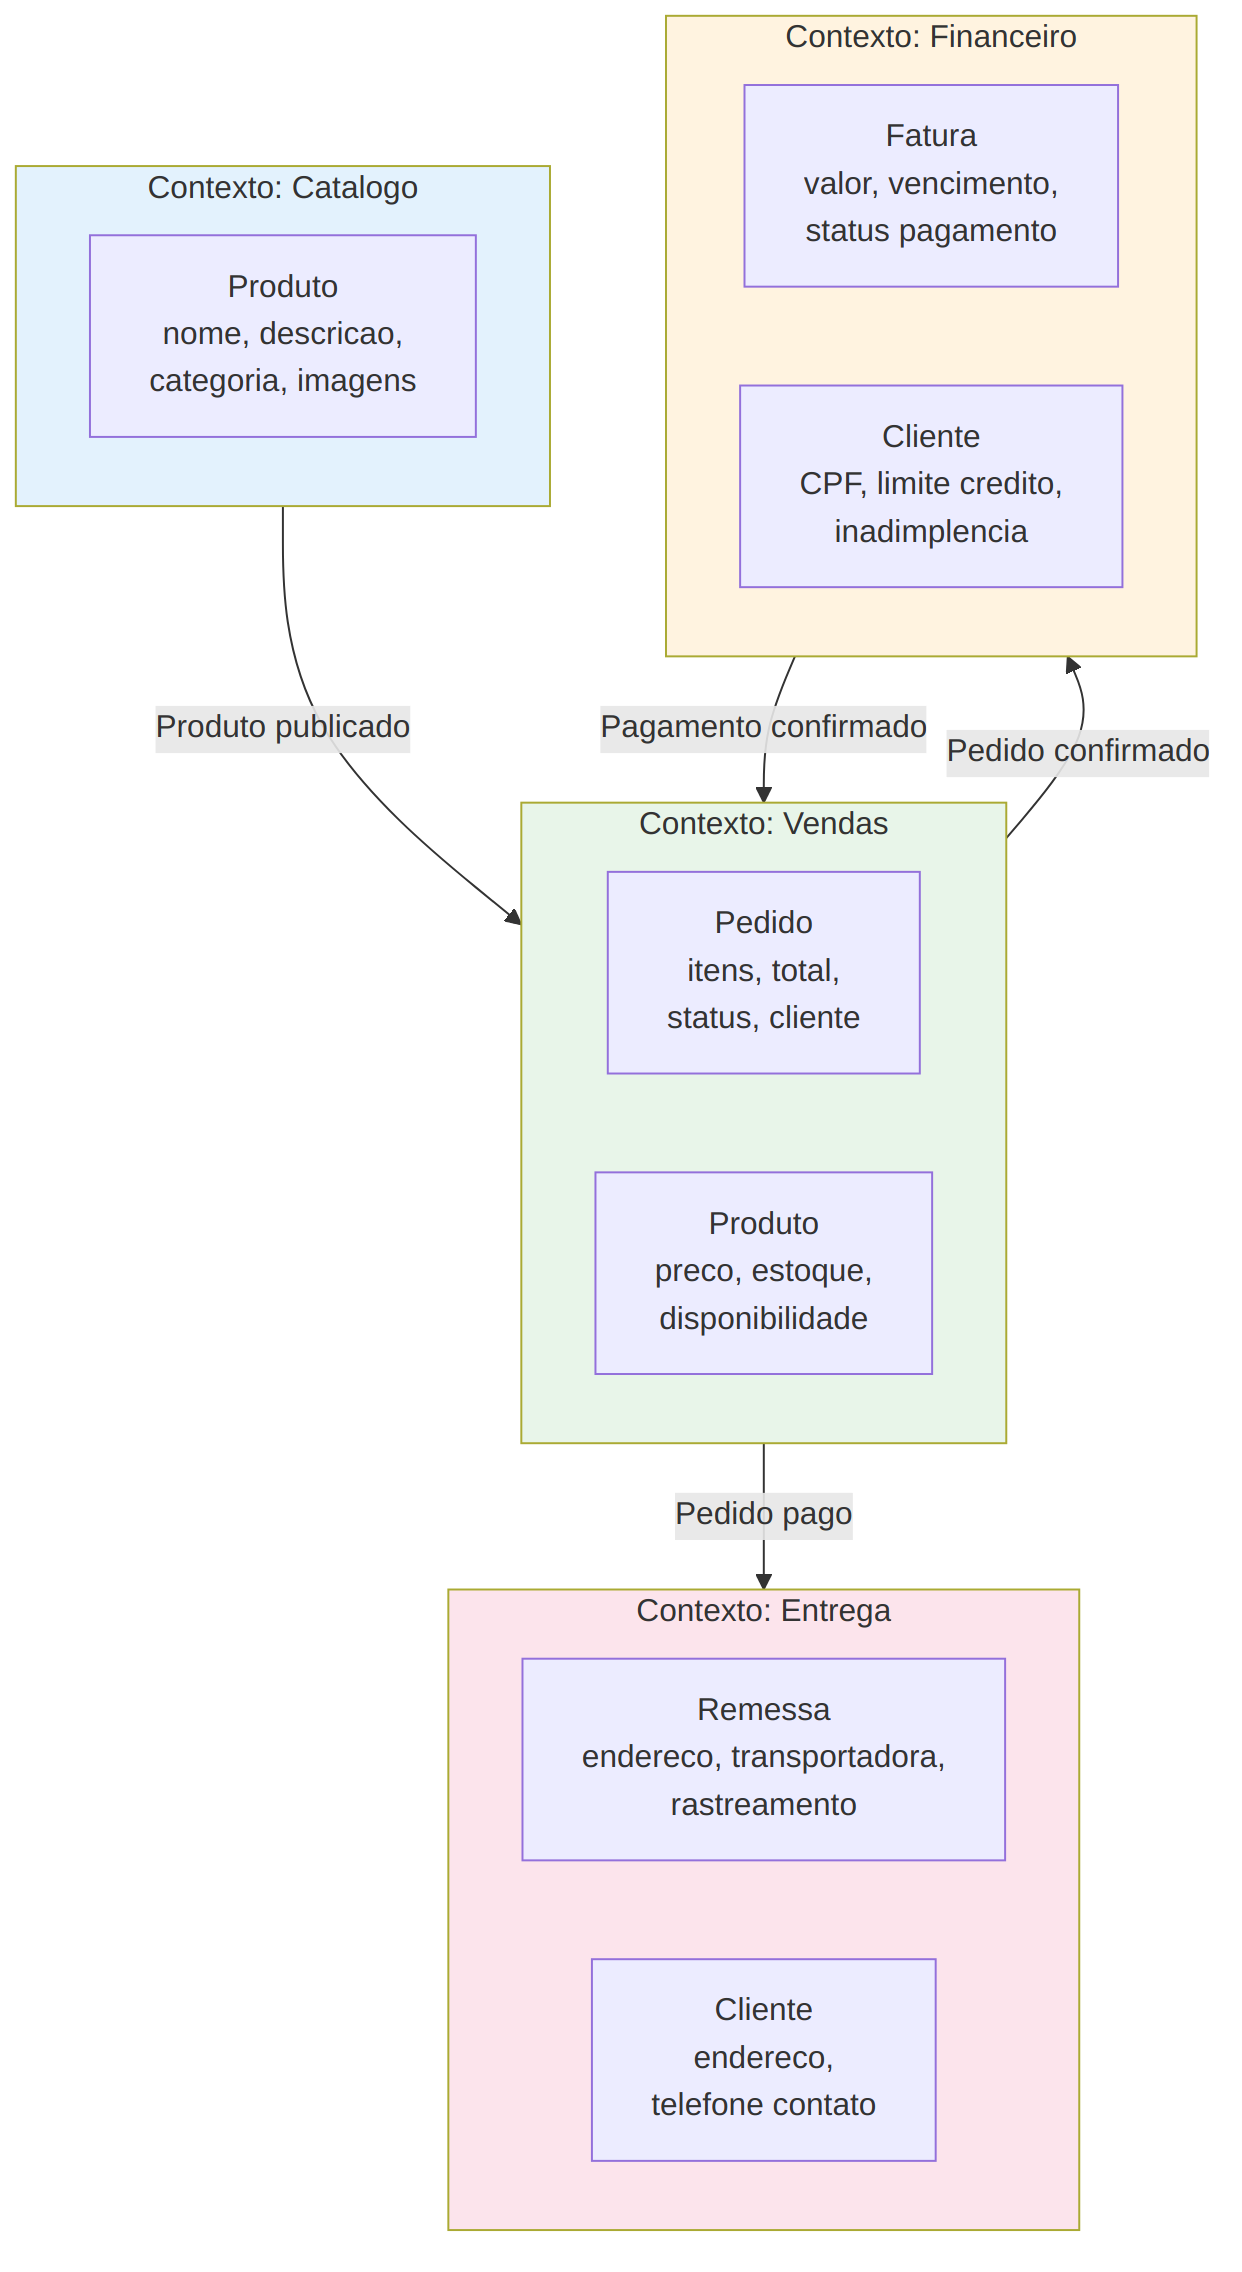
\includegraphics[width=0.85\textwidth]{imagens/02-arquitetura-antes-do-codigo-04-mermaid-bounded-contexts-de-um-e-commerce.png}
    \caption{Mermaid -- Bounded Contexts de um E-commerce}
\end{figure}

Observe como ``Produto'' e ``Cliente'' aparecem em múltiplos contextos, mas com
atributos diferentes em cada um. No contexto de Catálogo, um Produto tem nome,
descrição, fotos e categorias. No contexto de Estoque, o mesmo Produto tem
quantidade disponível, localização no armazém e ponto de reposição. No contexto
de Vendas, o Produto tem preço, descontos aplicáveis e margem de lucro. São
representações diferentes da mesma entidade do mundo real, cada uma otimizada
para as necessidades do seu contexto. A comunicação entre contextos acontece
via eventos de domínio (``Pedido confirmado'', ``Pagamento confirmado''), nunca
via acesso direto ao banco de dados do outro contexto.

Bounded contexts são a ponte entre DDD e arquitetura. Cada bounded context é um
candidato natural a ser um módulo em um monolito modular, ou um serviço em uma
arquitetura de microsserviços. As fronteiras dos bounded contexts são as
fronteiras naturais de deployment, porque dentro de cada contexto as mudanças
são frequentes e interdependentes, enquanto entre contextos as mudanças são
menos frequentes e mediadas por contratos estáveis (eventos, APIs).

\subsection{Entidades, Value Objects e Agregados}

No coração de cada bounded context, o DDD oferece padrões táticos para
modelar os conceitos do domínio de forma precisa. Esses padrões (Entidades,
Value Objects e Agregados) podem parecer abstratos à primeira vista, mas
correspondem a distinções fundamentais que existem em qualquer domínio de
negócio.

\textbf{Entidades} são objetos com identidade que persiste ao longo do tempo.
Um Pedido é uma entidade: mesmo que todos os seus atributos mudem (itens
adicionados, status alterado, endereço atualizado), ele continua sendo o mesmo
Pedido, identificado pelo seu ID. Pense em uma pessoa: ao longo da vida, seu
nome pode mudar (casamento), seu endereço muda várias vezes, sua aparência
física se transforma, mas ela continua sendo a mesma pessoa, com o mesmo
CPF. Essa persistência de identidade é o que define uma entidade. No código,
duas entidades são iguais se e somente se têm o mesmo identificador, independente
de seus outros atributos.

\textbf{Value Objects} são objetos definidos exclusivamente por seus atributos,
sem identidade própria. Um CPF é um Value Object: dois CPFs com o mesmo número
são iguais, ponto. Não faz sentido perguntar ``qual dos dois CPFs 123.456.789-00
é este?''. Eles são o mesmo. Um Endereco é um Value Object: se todos os campos
são idênticos (rua, número, cidade, CEP), são o mesmo endereço. Não importa
``quando'' o endereço foi criado ou ``por quem''; se os valores são iguais,
os objetos são iguais. Value Objects devem ser imutáveis: em vez de mudar o CEP
de um endereço, cria-se um novo endereço com o CEP correto. Essa imutabilidade
elimina toda uma classe de bugs relacionados a estado compartilhado.

Para entender a diferença concretamente, considere uma nota de R\$~50. A nota
em si é uma entidade: ela tem um número serial único, e se você perde \textit{aquela}
nota específica, não pode substituí-la por outra. Porém, o \textit{valor} de
R\$~50 é um Value Object: qualquer nota de R\$~50 serve igualmente para pagar
uma conta de R\$~50. Quando modelamos dinheiro em software, o que geralmente
nos importa é o valor (Value Object), não a nota física (entidade).

\textbf{Agregados} são clusters de entidades e value objects que mudam juntos
como uma unidade de consistência. O Pedido e seus Itens formam um agregado: não
faz sentido adicionar um item ao pedido sem passar pela lógica do Pedido (que
verifica estoque, calcula total, aplica descontos). Se um código externo pudesse
adicionar itens diretamente à lista de itens, sem passar pelo Pedido, as regras
de negócio poderiam ser violadas. Um item poderia ser adicionado a um pedido
já fechado, ou o total poderia ficar inconsistente com a soma dos itens.

O agregado define a fronteira transacional: tudo dentro de um agregado é
consistente a todo momento; entre agregados, a consistência pode ser eventual.
O Pedido é a ``raiz do agregado'': toda interação externa com os itens do
pedido deve passar pelo Pedido. Isso é mais do que uma questão de organização
de código. É uma garantia de integridade. O Pedido ``sabe'' suas regras de
negócio e as impõe, protegendo seus componentes internos de manipulação
indevida.

Uma analogia útil é a de um time de futebol. O técnico (raiz do agregado) é o
ponto de contato com o mundo externo. Se a diretoria quer escalar um jogador,
ela fala com o técnico, não vai diretamente ao jogador. O técnico decide se a
escalação faz sentido dentro da sua estratégia (regras de negócio). Os jogadores
(entidades internas) e a formação tática (value objects) são gerenciados pelo
técnico como uma unidade coesa.

\subsection{Domain Events}

Eventos de domínio representam algo que \textbf{aconteceu} no domínio e que
pode interessar a outras partes do sistema. Eles são escritos no passado:
\texttt{PedidoFoiPago}, \texttt{EstoqueFoiReservado}, \texttt{ClienteFoiCadastrado}.
Essa convenção de nomenclatura no passado não é arbitrária. Ela reflete a
natureza fundamental dos eventos: são fatos imutáveis. Uma vez que um pedido
foi pago, esse fato não pode ser ``desfeito''; pode ser compensado (com um
estorno), mas o evento original permanece verdadeiro. O pedido \textit{foi} pago
naquele momento.

A importância dos eventos de domínio vai além da comunicação técnica: eles tornam
a lógica de negócio explícita. Quando o código diz ``publique o evento
PedidoFoiPago'', qualquer pessoa (técnica ou não) entende o que está
acontecendo. Compare com ``chame o endpoint POST /api/v2/orders/\{id\}/status com
body \{status: paid\}'': a semântica se perde no mecanismo. No primeiro caso,
o que aconteceu no domínio é evidente. No segundo, é preciso decodificar URLs e
payloads para entender o que está acontecendo.

Eventos de domínio são também a base para padrões avançados como Event Sourcing,
onde o estado de uma entidade não é armazenado diretamente, mas reconstruído a
partir da sequência de eventos que aconteceram com ela. Em vez de armazenar
``saldo da conta = R\$~1.000'', armazena-se a sequência ``conta criada com
R\$~0'', ``depósito de R\$~500'', ``depósito de R\$~800'', ``saque de R\$~300''.
O saldo atual é calculado ``replayando'' os eventos. Esse padrão oferece
auditoria completa (todo histórico é preservado), capacidade de reconstruir
o estado em qualquer ponto do passado, e a possibilidade de corrigir bugs
reprocessando eventos com lógica corrigida.

Com o entendimento dos building blocks do DDD, surge uma pergunta prática:
como descobrimos quais são os eventos, as entidades e os bounded contexts do
nosso domínio? É aqui que entra o Event Storming, uma técnica de workshop que
transforma a descoberta do domínio em uma atividade colaborativa e visual.


\section{Event Storming: Descoberta Colaborativa do Domínio}

Event Storming é uma técnica de workshop criada por Alberto Brandolini em 2013
para explorar o domínio de negócio de forma colaborativa. Diferente de técnicas
tradicionais de levantamento de requisitos (onde um analista entrevista
stakeholders e produz documentos que ninguém lê), o Event Storming coloca
todos na mesma sala, com sticky notes e uma parede grande, e constrói um
entendimento compartilhado do domínio em poucas horas.

A motivação de Brandolini era resolver um problema que ele observava
repetidamente em projetos de software: o conhecimento do domínio estava
fragmentado entre múltiplas pessoas, e nenhuma delas tinha a visão completa.
O especialista de negócio entendia as regras, mas não sabia como elas se
conectavam com a tecnologia. O arquiteto entendia os padrões técnicos, mas
não compreendia as nuances do negócio. O developer entendia o código, mas
não sabia por que certas regras existiam. O Event Storming foi desenhado
para forçar essas perspectivas a colidirem, gerando um entendimento mais
completo do que qualquer indivíduo teria sozinho.

\subsection{Como Funciona}

O workshop segue uma progressão estruturada que é ao mesmo tempo simples o
suficiente para ser facilitada sem treinamento extensivo e rica o suficiente
para revelar complexidades ocultas no domínio. Vamos percorrer cada fase
como se estivéssemos participando de uma sessão real.

Na primeira fase, chamada de ``Event Generation'' ou tempestade de eventos,
os participantes (engenheiros, product owners, especialistas de domínio,
designers) recebem blocos de sticky notes laranjas e canetas grossas.
A instrução é simples: ``Escrevam tudo que acontece no sistema, no passado.''
As pessoas escrevem freneticamente: ``Pedido foi criado'', ``Pagamento foi
recusado'', ``Estoque ficou zerado'', ``Cliente cancelou assinatura'',
``Relatório mensal foi gerado'', ``Conta foi bloqueada por fraude''. Não há
julgamento nessa fase. O objetivo é gerar volume. Se alguém escreve algo
que parece ``errado'' ou ``fora de escopo'', ninguém corrige. Duplicatas são
bem-vindas. O único requisito é que o texto esteja no passado, representando
algo que já aconteceu. Essa fase tipicamente dura de 15 a 30 minutos e gera
entre 50 e 200 sticky notes, dependendo da complexidade do domínio.

Na segunda fase, os eventos são organizados em ordem cronológica na parede.
Essa é a fase mais reveladora, porque é quando os participantes começam a
discutir. ``Espera, o pagamento é confirmado antes ou depois do estoque ser
reservado?'' ``O que acontece se o pagamento for recusado depois do estoque
já ter sido reservado?'' ``Existe uma verificação de fraude? Quando ela
acontece?'' Padrões emergem naturalmente: cadeias de causa e efeito,
bifurcações onde o fluxo pode seguir caminhos diferentes, loops onde
processos se repetem. Gaps no conhecimento ficam visíveis (``o que
acontece entre o pagamento ser confirmado e o produto ser enviado?'') e
são marcados com sticky notes vermelhas, chamadas de ``hot spots''. Esses
hot spots são ouro: representam áreas do domínio onde o conhecimento é
incompleto, ambíguo ou contraditório, e que precisam de investigação adicional.

Na terceira fase, comandos são adicionados em sticky notes azuis: as ações
que disparam os eventos. ``Cliente clica em Comprar'' é o comando que
dispara ``Pedido foi criado''. ``Sistema verifica estoque'' é o comando que
dispara ``Estoque foi reservado'' ou ``Estoque insuficiente''. Essa fase
revela a causalidade do sistema: para cada evento, existe um comando que o
causou, e para cada comando, existem condições que o tornaram possível ou
impossível. As condições são representadas em sticky notes amarelas,
chamadas de ``policies'' ou ``regras de negócio'': ``somente clientes com
cadastro completo podem fazer pedidos'', ``pedidos acima de R\$~10.000
requerem aprovação do gerente''.

Na quarta fase, agregados são identificados: agrupamentos de eventos e
comandos que pertencem à mesma entidade de domínio. Olhando para a parede,
fica claro que ``Pedido foi criado'', ``Item foi adicionado ao pedido'',
``Pedido foi confirmado'' e ``Pedido foi cancelado'' todos orbitam em torno
do conceito de Pedido. Eles formam um agregado. Da mesma forma, ``Pagamento
foi iniciado'', ``Pagamento foi autorizado'' e ``Pagamento foi recusado''
formam o agregado de Pagamento. Os bounded contexts emergem dos agrupamentos
de agregados: agregados que interagem frequentemente entre si provavelmente
pertencem ao mesmo bounded context, enquanto agregados que se comunicam
apenas via eventos provavelmente pertencem a bounded contexts diferentes.

\subsection{Por que Funciona}

Event Storming é eficaz porque inverte o processo tradicional. Em vez de começar
com entidades e atributos (``quais são os campos do Cliente?''), começa com
comportamento (``o que acontece no sistema?''). Isso alinha o modelo de software
com a realidade do negócio, porque negócios são feitos de \textbf{coisas que
acontecem}, não de tabelas de banco de dados.

Quando um empresário descreve seu negócio, ele não fala em termos de tabelas e
campos. Ele fala em termos de processos: ``o cliente faz um pedido, nós
verificamos o estoque, processamos o pagamento, e enviamos o produto.'' O Event
Storming captura exatamente essa linguagem processual e a transforma em um
modelo que pode ser diretamente implementado em código. Não há tradução
necessária entre a linguagem do negócio e a linguagem do software: elas
são a mesma.

O formato de workshop também elimina o jogo de telefone entre stakeholders
e engenheiros. Quando o especialista de domínio e o arquiteto estão na mesma
parede, discordâncias e ambiguidades são resolvidas na hora, não três sprints
depois, quando o código já foi escrito baseado em premissas erradas. O custo
de resolver uma ambiguidade durante um workshop é de minutos. O custo de
resolver a mesma ambiguidade após a implementação é de dias ou semanas. E o
custo de descobrir a ambiguidade em produção, quando um bug afeta clientes
reais, é incalculável.

Outro benefício frequentemente subestimado do Event Storming é o alinhamento
do time. Após uma sessão de duas a quatro horas, todos os participantes
compartilham o mesmo modelo mental do domínio. Não há mais ``o que o Pedro
entende sobre o fluxo de pagamento'' versus ``o que a Maria entende sobre o
fluxo de pagamento''. Há um modelo compartilhado, visível na parede, que
todos ajudaram a construir. Esse alinhamento reduz dramaticamente os
mal-entendidos durante o desenvolvimento subsequente.

A descoberta colaborativa do domínio via Event Storming naturalmente leva à
pergunta: onde colocamos o domínio no código? Como garantimos que a lógica de
negócio descoberta no workshop não se perca em meio a detalhes de infraestrutura?
A resposta está na arquitetura hexagonal.


\section{Arquitetura Hexagonal: Portas e Adaptadores}

A arquitetura hexagonal, proposta por Alistair Cockburn em 2005, é um dos padrões
arquiteturais mais influentes da engenharia de software moderna. Sua premissa
central é simples e poderosa: o domínio do negócio não deve depender de nenhuma
tecnologia externa. O domínio não sabe que existe HTTP, não sabe que existe
PostgreSQL, não sabe que existe Kafka. Ele define \textbf{portas} (interfaces) que
descrevem o que precisa do mundo externo, e \textbf{adaptadores} implementam
essas portas usando tecnologias concretas.

A motivação de Cockburn era resolver um problema que ele observava repetidamente
em projetos de software: a lógica de negócio estava tão entrelaçada com
detalhes de infraestrutura que era impossível testá-la isoladamente, e trocar
qualquer componente técnico exigia reescrever grandes porções do sistema.
Cockburn percebeu que o problema era de dependência: a lógica de negócio
\textit{dependia} da infraestrutura, quando deveria ser o contrário. A
infraestrutura deveria depender da lógica de negócio, adaptando-se a ela
como um encaixe.

O nome ``hexagonal'' não tem significado matemático especial. Cockburn
escolheu o hexágono porque precisava de uma forma geométrica com múltiplas
faces para representar as múltiplas portas do sistema. Poderia ter sido um
octágono ou um decágono. A forma hexagonal ficou, e o nome pegou. Nos anos
subsequentes, outros nomes surgiram para padrões muito similares: ``Ports
and Adapters'' (o próprio Cockburn prefere este nome), ``Onion Architecture''
(proposta por Jeffrey Palermo em 2008), e ``Clean Architecture'' (proposta
por Robert C. Martin em 2012). As diferenças entre eles são menores do que
as semelhanças: todos colocam o domínio no centro, livre de dependências
externas.

\begin{figure}[htbp]
    \centering
    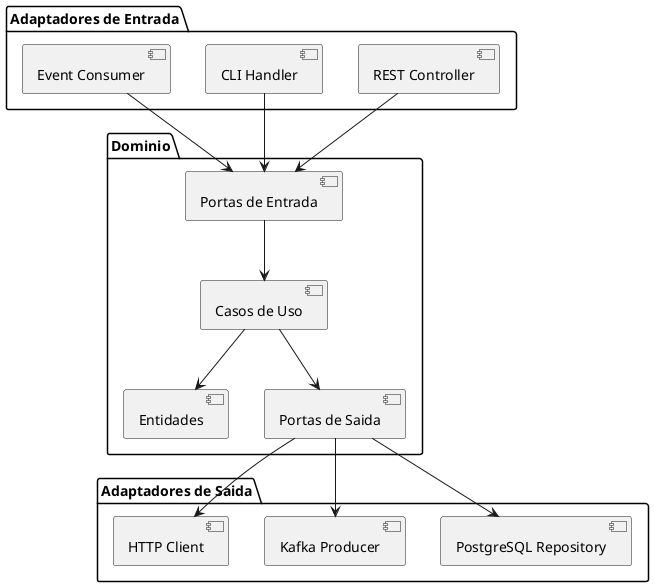
\includegraphics[width=0.85\textwidth]{imagens/02-arquitetura-antes-do-codigo-05-arquitetura-hexagonal-portas-e-adaptadores.png}
    \caption{Arquitetura Hexagonal -- Portas e Adaptadores}
\end{figure}

Na arquitetura hexagonal, existem dois tipos de portas. As \textbf{portas de
entrada} (ou ``driving ports'') definem como o mundo externo pode interagir
com o domínio. Elas são as operações que o sistema oferece: ``criar pedido'',
``cancelar assinatura'', ``transferir dinheiro''. As \textbf{portas de saída}
(ou ``driven ports'') definem o que o domínio precisa do mundo externo:
``buscar conta por ID'', ``salvar transação'', ``publicar evento'',
``enviar e-mail''.

Para cada porta, existem um ou mais \textbf{adaptadores}. Um adaptador de
entrada traduz uma solicitação do mundo externo para uma chamada ao domínio:
o adaptador HTTP recebe uma requisição REST e chama o caso de uso ``transferir
dinheiro''. O adaptador de CLI recebe argumentos de linha de comando e chama o
mesmo caso de uso. O adaptador de evento recebe uma mensagem do Kafka e chama
o mesmo caso de uso. Do ponto de vista do domínio, não importa \textit{como} a
solicitação chegou; importa apenas \textit{o que} foi solicitado.

Da mesma forma, um adaptador de saída implementa uma porta de saída usando
uma tecnologia concreta: o adaptador PostgreSQL implementa a porta
``repositório de contas'' usando SQL. O adaptador DynamoDB implementa a
mesma porta usando a API da Amazon. O adaptador em memória implementa a
mesma porta usando um dicionário Python, o que é perfeito para testes. Todos
satisfazem o mesmo contrato, permitindo que sejam intercambiáveis.

A beleza dessa arquitetura está na testabilidade e na adaptabilidade. Para testar
a lógica de negócio, basta criar adaptadores falsos (mocks ou stubs) que
implementam as portas de saída. Para trocar o banco de dados de PostgreSQL para
DynamoDB, basta criar um novo adaptador, e o domínio não muda uma linha sequer.
Para adicionar uma nova forma de entrada (um chatbot, por exemplo, além da API
REST), basta criar um novo adaptador de entrada. Novamente, o domínio
permanece intocado.

\subsection{Implementação em Python}

Vamos ver uma implementação concreta da arquitetura hexagonal em Python. O
exemplo é um sistema simples de transferência bancária. Esse exemplo é
deliberadamente simples para que o padrão fique claro, mas os mesmos princípios
se aplicam a domínios de qualquer complexidade.

Primeiro, as entidades e value objects do domínio:

\begin{lstlisting}[language=Python, caption={Domínio -- Entidades e Value Objects}]
from dataclasses import dataclass
from decimal import Decimal
from uuid import UUID, uuid4

@dataclass(frozen=True)
class Dinheiro:
    """Value Object imutavel representando um valor monetario."""
    valor: Decimal
    moeda: str = "BRL"

    def __post_init__(self):
        if self.valor < 0:
            raise ValueError("Valor monetario nao pode ser negativo")

@dataclass
class Conta:
    """Entidade com identidade -- a conta bancaria."""
    id: UUID
    titular: str
    saldo: Dinheiro

    def debitar(self, quantia: Dinheiro) -> None:
        if quantia.valor > self.saldo.valor:
            raise ValueError("Saldo insuficiente")
        self.saldo = Dinheiro(self.saldo.valor - quantia.valor)

    def creditar(self, quantia: Dinheiro) -> None:
        self.saldo = Dinheiro(self.saldo.valor + quantia.valor)
\end{lstlisting}

Observe como o \texttt{Dinheiro} é um Value Object (imutável, definido por
seus atributos) e a \texttt{Conta} é uma Entidade (tem identidade via
\texttt{id}). A lógica de negócio está nas entidades: a \texttt{Conta} sabe
como se debitar e se creditar, e impõe suas invariantes (saldo não pode ficar
negativo). Nenhuma dessas classes sabe nada sobre banco de dados, HTTP, ou
qualquer tecnologia externa.

Agora, as portas, interfaces que definem \textit{o que} o domínio precisa,
sem definir \textit{como}:

\begin{lstlisting}[language=Python, caption={Portas -- Interfaces do Domínio}]
from abc import ABC, abstractmethod

class RepositorioDeConta(ABC):
    """Porta de saida: como o dominio persiste contas."""

    @abstractmethod
    def buscar_por_id(self, conta_id: UUID) -> Conta:
        ...

    @abstractmethod
    def salvar(self, conta: Conta) -> None:
        ...

class PublicadorDeEventos(ABC):
    """Porta de saida: como o dominio publica eventos."""

    @abstractmethod
    def publicar(self, evento: dict) -> None:
        ...
\end{lstlisting}

O caso de uso (a lógica de negócio propriamente dita) depende apenas das portas,
nunca de implementações concretas:

\begin{lstlisting}[language=Python, caption={Caso de Uso -- Transferência Bancária}]
class TransferirDinheiro:
    """Caso de uso: transferir dinheiro entre contas."""

    def __init__(
        self,
        repositorio: RepositorioDeConta,
        publicador: PublicadorDeEventos,
    ):
        self.repositorio = repositorio
        self.publicador = publicador

    def executar(
        self, origem_id: UUID, destino_id: UUID, quantia: Dinheiro
    ) -> None:
        origem = self.repositorio.buscar_por_id(origem_id)
        destino = self.repositorio.buscar_por_id(destino_id)

        origem.debitar(quantia)
        destino.creditar(quantia)

        self.repositorio.salvar(origem)
        self.repositorio.salvar(destino)

        self.publicador.publicar({
            "tipo": "TransferenciaRealizada",
            "origem": str(origem_id),
            "destino": str(destino_id),
            "valor": str(quantia.valor),
        })
\end{lstlisting}

Finalmente, os adaptadores, ou seja, as implementações concretas que conectam o domínio
ao mundo real:

\begin{lstlisting}[language=Python, caption={Adaptadores -- Implementações Concretas}]
import json
from kafka import KafkaProducer

class ContaPostgresRepository(RepositorioDeConta):
    """Adaptador de saida: persiste contas no PostgreSQL."""

    def __init__(self, connection):
        self.conn = connection

    def buscar_por_id(self, conta_id: UUID) -> Conta:
        cursor = self.conn.cursor()
        cursor.execute(
            "SELECT id, titular, saldo FROM contas WHERE id = %s",
            (str(conta_id),)
        )
        row = cursor.fetchone()
        return Conta(
            id=UUID(row[0]),
            titular=row[1],
            saldo=Dinheiro(Decimal(str(row[2]))),
        )

    def salvar(self, conta: Conta) -> None:
        cursor = self.conn.cursor()
        cursor.execute(
            "UPDATE contas SET saldo = %s WHERE id = %s",
            (str(conta.saldo.valor), str(conta.id)),
        )
        self.conn.commit()

class KafkaPublicadorDeEventos(PublicadorDeEventos):
    """Adaptador de saida: publica eventos no Kafka."""

    def __init__(self, bootstrap_servers: str):
        self.producer = KafkaProducer(
            bootstrap_servers=bootstrap_servers,
            value_serializer=lambda v: json.dumps(v).encode(),
        )

    def publicar(self, evento: dict) -> None:
        self.producer.send("eventos-dominio", value=evento)
        self.producer.flush()
\end{lstlisting}

O ponto crucial é que o caso de uso \texttt{TransferirDinheiro} funciona
igualmente com um banco PostgreSQL real, com um repositório em memória para
testes, ou com um banco DynamoDB na nuvem. A lógica de negócio está isolada
e protegida. Essa proteção não é apenas uma conveniência de design; é uma
garantia de longevidade. Tecnologias de banco de dados e mensageria mudam
a cada poucos anos. A lógica de negócio de uma transferência bancária não
mudou em séculos. Ao separar as duas, garantimos que a parte estável do
sistema (o domínio) não é contaminada pela parte volátil (a infraestrutura).

A arquitetura hexagonal nos dá a estrutura para proteger o domínio. Mas
quando tomamos uma decisão arquitetural (como usar arquitetura hexagonal),
precisamos registrar essa decisão e suas razões. É exatamente para isso
que servem os Architecture Decision Records.


\section{Decisões Arquiteturais e ADRs}

Toda arquitetura é o resultado de um conjunto de decisões. O problema é que,
sem documentação, essas decisões se perdem. Três meses depois, ninguém lembra
por que o Kafka foi escolhido em vez do RabbitMQ. Um ano depois, um novo
engenheiro questiona a decisão e propõe migrar, sem saber que a escolha original
foi motivada pela necessidade de replay de eventos, uma necessidade que
continua existindo. Dois anos depois, o mesmo debate acontece novamente, consumindo
horas de reunião para chegar à mesma conclusão que já havia sido alcançada antes.

Esse ciclo de amnésia organizacional é extraordinariamente comum e
extraordinariamente caro. Michael Nygard, um engenheiro e consultor com décadas
de experiência, observou esse padrão em inúmeras organizações e propôs uma
solução elegante por volta de 2011: o Architecture Decision Record (ADR). A
ideia é desarmantemente simples, tão simples que muitas pessoas a descartam
por acharem que ``algo tão simples não pode resolver um problema tão grande''.
Mas a simplicidade é justamente a razão do seu sucesso.

O ADR é um documento curto, armazenado no repositório junto do código, que
captura o contexto, a decisão e suas consequências. Cada ADR é numerado
sequencialmente (ADR-001, ADR-002, ...) e nunca é deletado ou editado
retroativamente. Se uma decisão é substituída, o ADR original recebe o
status ``substituída por ADR-XXX'', e um novo ADR é criado explicando por
que a decisão mudou. Isso cria um registro histórico completo e auditável
da evolução arquitetural do sistema.

O que acontece com times que não usam ADRs é previsível e triste. As decisões
vivem apenas nas cabeças das pessoas que as tomaram. Quando essas pessoas saem
da empresa (e eventualmente saem), o conhecimento vai com elas. Os engenheiros
que ficam herdam um sistema cujas decisões não entendem, e vivem com medo de
mudar qualquer coisa ``porque deve ter um motivo para estar assim''. O resultado
é paralisia: o sistema para de evoluir, não porque a mudança seja tecnicamente
difícil, mas porque ninguém tem confiança para decidir o que mudar. ADRs
resolvem esse problema ao tornar o raciocínio por trás de cada decisão
acessível a qualquer pessoa, em qualquer momento.

\subsection{Estrutura de um ADR}

Um ADR tem quatro seções essenciais, cada uma servindo um propósito específico
na preservação do conhecimento arquitetural.

A seção de \textbf{Contexto} descreve o problema ou a necessidade que motivou a
decisão. Quais restrições existiam no momento (técnicas, organizacionais,
regulatórias, de prazo)? Qual era o estado do sistema? Essa seção é crucial porque
a adequação de uma decisão depende do contexto. Uma decisão que era perfeita há
dois anos pode ser inadequada hoje, mas só é possível avaliar isso se o contexto
original estiver registrado. Sem o contexto, não se pode distinguir uma decisão
que ``era boa na época mas o contexto mudou'' de uma decisão que ``sempre foi
ruim''.

A seção de \textbf{Decisão} registra o que foi decidido. Crucialmente, ela também
lista as alternativas que foram consideradas e por que foram descartadas. Essa
lista de alternativas rejeitadas é tão valiosa quanto a decisão em si, porque
evita que futuros engenheiros percam tempo avaliando opções que já foram
investigadas e descartadas por boas razões. Se a alternativa ``usar RabbitMQ''
foi descartada porque não suporta replay de eventos, e essa necessidade continua
existindo, nenhum tempo precisa ser gasto reavaliando RabbitMQ.

A seção de \textbf{Consequências} documenta o que se ganha e o que se perde com
a decisão. Toda decisão arquitetural é um trade-off, e ser honesto sobre o que
se perde é tão importante quanto celebrar o que se ganha. Se a escolha do Kafka
traz replay de eventos mas também traz uma curva de aprendizado íngreme e custos
operacionais maiores, ambos devem ser registrados. Essa honestidade permite que
futuros leitores avaliem se os trade-offs ainda são aceitáveis.

A seção de \textbf{Status} indica o estado atual da decisão: proposta (ainda em
discussão), aceita (implementada e ativa), obsoleta (já não se aplica), ou
substituída por ADR-XXX (uma nova decisão tomou seu lugar).

\subsection{Template de ADR}

\begin{lstlisting}[language={}, caption={Template de ADR em Markdown}]
# ADR-001: Usar Kafka como barramento de eventos

## Status
Aceita (2024-03-15)

## Contexto
O sistema de pedidos precisa comunicar eventos para os servicos
de estoque, notificacao e analytics. A comunicacao precisa ser
assincrona para nao acoplar os servicos temporalmente.

Requisitos identificados:
- Replay de eventos para reprocessamento
- Retencao de 30 dias para auditoria
- Throughput de ~10.000 eventos/segundo no pico
- Ordenacao garantida por pedido (partition key)

## Alternativas Consideradas
1. **RabbitMQ**: mais simples de operar, mas sem replay nativo
   e retencao limitada.
2. **Amazon SQS + SNS**: gerenciado, mas sem ordenacao garantida
   e replay impossivel.
3. **Apache Kafka**: replay nativo, retencao configuravel,
   ordenacao por particao, ecossistema maduro.

## Decisao
Usar Apache Kafka (gerenciado via Confluent Cloud).

## Consequencias
### Positivas
- Replay de eventos para reprocessamento e debug
- Retencao configuravel (30 dias para auditoria)
- Ordenacao por partition key (ID do pedido)
- Ecossistema rico (Kafka Streams, Connect, Schema Registry)

### Negativas
- Curva de aprendizado maior que RabbitMQ
- Custo operacional mais alto (Confluent Cloud ~$800/mes)
- Complexidade de configuracao de particoes e replicacao
- Time precisa aprender conceitos de consumer groups e offsets
\end{lstlisting}

\subsection{Fluxo de Decisão Arquitetural}

Uma decisão arquitetural não surge do nada. Ela nasce de uma necessidade ou
problema identificado, passa por uma fase de investigação e discussão, e
culmina em um registro formal. O diagrama a seguir ilustra o processo
recomendado para tomar e registrar decisões arquiteturais:

\begin{figure}[htbp]
    \centering
    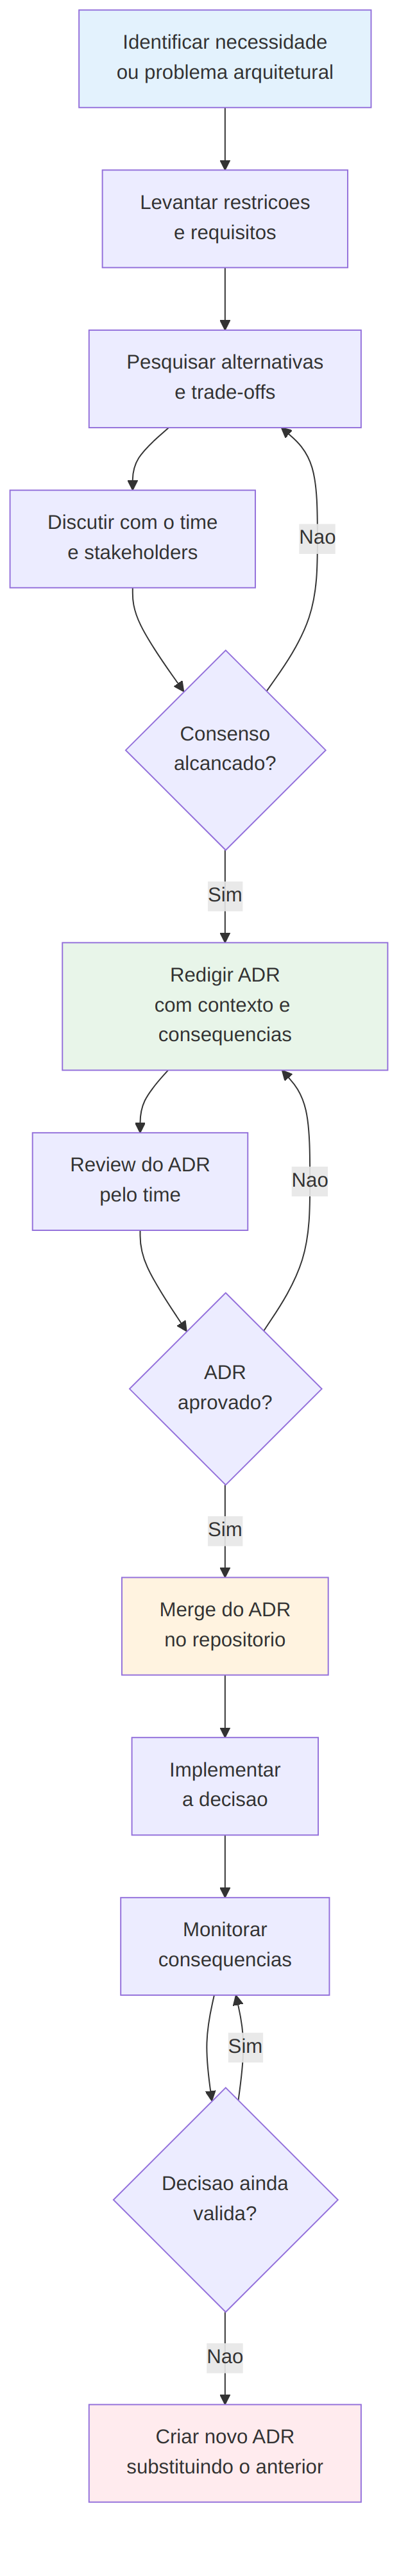
\includegraphics[width=0.85\textwidth]{imagens/02-arquitetura-antes-do-codigo-06-mermaid-fluxo-de-decisao-arquitetural-com-adr.png}
    \caption{Mermaid -- Fluxo de Decisão Arquitetural com ADR}
\end{figure}

ADRs devem ser armazenados no repositório do projeto, em um diretório dedicado
como \texttt{docs/adr/}. Isso garante que eles versionem junto com o código,
sejam revisáveis via pull request, e estejam acessíveis a qualquer engenheiro
que precise entender o histórico de decisões. Quando um novo membro entra no
time, uma das primeiras coisas que deveria fazer é ler os ADRs do projeto:
eles contam a história das decisões que moldaram o sistema atual, fornecendo
contexto que nenhuma documentação de API ou diagrama de arquitetura pode
oferecer.

Existe uma prática particularmente valiosa que algumas equipes adotam: o
``ADR review'' periódico. A cada trimestre, o time revisa os ADRs existentes
e avalia se o contexto mudou o suficiente para justificar uma revisão de
alguma decisão. Isso evita a inércia arquitetural, a tendência de manter
decisões antigas não porque são as melhores, mas porque ninguém questionou.
O ADR review transforma a evolução arquitetural em um processo deliberado e
contínuo.

Com a capacidade de tomar e registrar decisões arquiteturais de forma
disciplinada, estamos prontos para abordar uma verdade fundamental da
engenharia de software: toda arquitetura precisa mudar. A questão não é se,
mas quando e como.


\section{Design para Mudança: Arquitetura Evolutiva}

A ideia de que se pode ``acertar a arquitetura de primeira'' é uma fantasia.
Todo sistema que sobrevive ao contato com a realidade precisa evoluir. O
desafio não é prever o futuro; é criar condições para que a mudança seja
barata quando inevitavelmente chegar.

Essa verdade é desconfortável para muitos engenheiros, especialmente os mais
experientes, que gostariam de acreditar que sua experiência permite prever o
que o sistema precisará em três, cinco ou dez anos. A realidade é que ninguém
consegue fazer essa previsão de forma confiável. Requisitos mudam porque o
mercado muda, regulamentações mudam, a estratégia da empresa muda, os
usuários descobrem usos inesperados para o sistema. A única certeza é que
as premissas de hoje serão parcialmente incorretas amanhã. Uma arquitetura
boa não é aquela que previu todas as mudanças, e sim aquela que acomoda
mudanças não previstas a um custo razoável.

\subsection{Fitness Functions: Testes Arquiteturais}

O conceito de fitness functions, popularizado pelo livro \textit{Building
Evolutionary Architectures} de Neal Ford, Rebecca Parsons e Patrick Kua
publicado em 2017, aplica a ideia de testes automatizados à própria
arquitetura. Assim como testes unitários verificam que o código funciona
corretamente, fitness functions verificam que a arquitetura está sendo
respeitada.

A motivação é simples: regras arquiteturais que existem apenas em
documentação ou na cabeça das pessoas são invariavelmente violadas com o
tempo. Um arquiteto pode decretar que ``o módulo de apresentação nunca deve
importar diretamente o módulo de acesso a dados'', mas se essa regra não é
verificada automaticamente, eventualmente alguém (pressionado por um
prazo, ou simplesmente desconhecendo a regra) vai criar a importação
proibida. E uma vez que a primeira violação passa, as demais seguem
rapidamente, num fenômeno conhecido como ``broken windows'' (janelas
quebradas). Fitness functions transformam regras arquiteturais em
verificações automatizadas que impedem violações antes que elas cheguem ao
código base.

Vejamos um exemplo concreto de fitness function. A verificação de dependência
entre módulos garante que a separação em camadas é respeitada, impedindo que
o módulo de apresentação importe diretamente o módulo de infraestrutura.

\begin{lstlisting}[language=Python, caption={Fitness Function -- Verificação de Dependências}]
import ast
import os

def verificar_dependencias_proibidas():
    """
    Fitness function: o modulo 'apresentacao' nao deve
    importar diretamente o modulo 'infraestrutura'.
    """
    violacoes = []
    diretorio = "src/apresentacao"

    for root, dirs, files in os.walk(diretorio):
        for arquivo in files:
            if not arquivo.endswith(".py"):
                continue
            caminho = os.path.join(root, arquivo)
            with open(caminho) as f:
                tree = ast.parse(f.read())

            for node in ast.walk(tree):
                if isinstance(node, ast.Import):
                    for alias in node.names:
                        if "infraestrutura" in alias.name:
                            violacoes.append(
                                f"{caminho}: import {alias.name}"
                            )
                elif isinstance(node, ast.ImportFrom):
                    if node.module and "infraestrutura" in node.module:
                        violacoes.append(
                            f"{caminho}: from {node.module}"
                        )

    assert not violacoes, (
        f"Violacoes de arquitetura encontradas:\n"
        + "\n".join(violacoes)
    )
\end{lstlisting}

Verificações de dependência são apenas um tipo de fitness function. O tempo de
resposta dos endpoints da API também pode
ser verificado automaticamente para garantir que nenhum endpoint leva mais
que 200ms para responder sob carga normal. Quando um novo endpoint é adicionado
ou uma mudança causa degradação de performance, a fitness function detecta o
problema antes que ele chegue a produção.

O tamanho de deployment é outro aspecto frequentemente monitorado. É surpreendentemente
comum que imagens Docker cresçam gradualmente à medida que dependências são
adicionadas sem que as antigas sejam removidas. Uma fitness function que verifica
que a imagem não ultrapassa 500MB previne esse ``bloat'' gradual que eventualmente
impacta tempos de deployment e custos de armazenamento.

A cobertura de testes por módulo é outra fitness function valiosa. Em vez de
exigir uma cobertura global uniforme (que frequentemente leva a testes
superficiais escritos apenas para atingir a métrica), define-se cobertura
diferenciada por criticidade: módulos críticos como pagamentos e autenticação
mantêm cobertura acima de 90\%, enquanto módulos menos críticos como
configurações de UI podem ter cobertura de 60\%.

A chave é que fitness functions rodam automaticamente, idealmente no pipeline
de CI/CD. Se uma mudança de código viola uma restrição arquitetural, o build
falha, assim como falharia se um teste unitário quebrasse. Isso transforma
regras arquiteturais de ``recomendações que todo mundo ignora'' em
``restrições que o sistema impõe''. A diferença é enorme: recomendações
dependem de disciplina individual, que varia entre pessoas e ao longo do
tempo. Restrições automatizadas são consistentes e implacáveis.

\subsection{Strangler Fig: Migração Gradual}

O Strangler Fig Pattern (nomeado em homenagem às figueiras estrangulantes que
crescem ao redor de árvores existentes até eventualmente substituí-las) é uma
estratégia de migração incremental. Em vez de reescrever um sistema legado do
zero (o famoso ``big bang'' que quase sempre falha), o Strangler Fig permite
migrar funcionalidade por funcionalidade, mantendo o sistema antigo em operação
durante todo o processo.

Martin Fowler cunhou o nome do padrão em 2004, inspirado por
figueiras estrangulantes que ele observou em viagens ao Queensland,
Austrália. Essas árvores germinam no topo de outra árvore, crescem raízes
que descem pelo tronco do hospedeiro, e eventualmente envolvem completamente
a árvore original. Quando o hospedeiro morre, a figueira permanece de pé,
sustentada por suas próprias raízes que tomaram a forma do tronco original.
É uma metáfora perfeita para a migração de sistemas legados.

A história da engenharia de software está repleta de projetos de reescrita
total que fracassaram espetacularmente. O caso mais famoso é provavelmente o
do Netscape Navigator: em 1998, a Netscape decidiu reescrever seu navegador
do zero. O projeto levou três anos, durante os quais o Internet Explorer da
Microsoft dominou o mercado. Quando o novo Netscape finalmente foi lançado,
era tarde demais. Joel Spolsky, em seu famoso artigo ``Things You Should
Never Do, Part I'', chamou a reescrita total de ``o pior erro estratégico
que uma empresa de software pode cometer''. O Strangler Fig existe como
antídoto para essa tentação.

O mecanismo é elegante: um proxy (ou API gateway) recebe todas as requisições e
decide para onde encaminhá-las. No início, 100\% do tráfego vai para o sistema
legado. À medida que novas funcionalidades são reimplementadas no sistema novo,
o proxy começa a direcionar as requisições correspondentes para o novo sistema.
Eventualmente, todo o tráfego migra e o sistema legado pode ser desligado.

As vantagens dessa abordagem são significativas. O risco é minimizado porque a
migração acontece em pequenos passos, cada um deles reversível. O sistema legado
continua funcionando durante toda a transição, então não há downtime planejado.
O time pode aprender e ajustar a estratégia durante o processo, em vez de
apostar tudo em um plano concebido antes de qualquer experiência prática com
o novo sistema. E o valor é entregue incrementalmente: cada funcionalidade
migrada traz benefícios imediatos, em vez de exigir que todo o trabalho
esteja completo antes que qualquer benefício se materialize.

Um exemplo real: imagine uma fintech que tem um monolito legado em Java responsável
por processamento de transações, gestão de contas e relatórios. A equipe decide
migrar para microsserviços. Em vez de reescrever tudo, eles começam pelo módulo
de relatórios (menos crítico), criam um novo serviço e configuram o gateway para
direcionar requisições de relatórios para ele. Após validar que funciona, migram
a gestão de contas. Por último, o processamento de transações. O monolito vai
``encolhendo'' enquanto o novo ecossistema vai ``crescendo'' ao redor dele.

A ordem de migração não é arbitrária. Geralmente começa-se pelos módulos menos
críticos e mais independentes, por três razões. Primeiro, o risco é menor:
se algo der errado com o módulo de relatórios, nenhuma transação é afetada.
Segundo, a equipe ganha experiência com o processo de migração antes de
enfrentar os módulos mais complexos. Terceiro, o sucesso inicial cria
confiança e momentum para as migrações subsequentes.

O padrão Strangler Fig ensina algo importante sobre a natureza da mudança
em software: grandes transformações são melhor executadas como uma série de
pequenas transformações incrementais. Esse princípio se aplica não apenas a
migrações de sistemas legados, mas a qualquer mudança arquitetural
significativa.


\section{Estudo de Caso: Arquitetando um Sistema Fintech}

Para consolidar os conceitos discutidos neste capítulo, vamos percorrer o processo
completo de design arquitetural de um sistema fintech fictício, mas realista: o
\textbf{PayFlow}, uma plataforma de pagamentos para pequenos comerciantes. Este
estudo de caso demonstra como os conceitos que discutimos separadamente se integram
quando aplicados juntos, cada um contribuindo para decisões que se reforçam mutuamente.

\subsection{Contexto do Negócio}

O PayFlow precisa oferecer: cadastro de comerciantes, processamento de
pagamentos via Pix e cartão de crédito, split de pagamentos (dividir o valor
entre múltiplos recebedores), dashboard de acompanhamento em tempo real, e
geração de relatórios fiscais. A expectativa inicial é de 500 comerciantes
e 50.000 transações por dia, com projeção de crescimento de 10x em 18 meses.

Esses números são importantes porque influenciam diretamente as decisões
arquiteturais. Cinquenta mil transações por dia equivalem a aproximadamente
35 transações por minuto em média, com picos que podem chegar a 200 por
minuto em horários de maior movimento. Esses números são perfeitamente
manejáveis por um monolito bem construído em uma única máquina. A projeção de
10x (500 mil transações por dia) também é manejável, embora comece a
justificar otimizações de performance e talvez separação de workloads de
leitura e escrita. Microsserviços, com toda sua complexidade operacional,
não se justificam para esses volumes, a menos que haja outras razões
além de performance.

\subsection{Event Storming do Domínio}

Realizamos um workshop de Event Storming com o time (product owner, dois
engenheiros, um especialista em compliance financeiro). Os principais eventos
identificados durante a sessão contam a história do domínio de forma
eloquente.

O fluxo começa com o onboarding do comerciante: o evento \textbf{ComercianteFoiCadastrado}
marca o início da relação, seguido por \textbf{DocumentacaoFoiVerificada} (o processo
de KYC, ou Know Your Customer, exigido por regulamentação financeira), que leva
a \textbf{ComercianteFoiAprovado} ou \textbf{ComercianteFoiRecusado}, dependendo da
conformidade documental.

Uma vez aprovado, o comerciante pode receber pagamentos. O evento
\textbf{PagamentoFoiIniciado} dispara quando um cliente do comerciante inicia uma
transação. O gateway de pagamento responde com \textbf{PagamentoFoiAutorizado}, seguido
por \textbf{PagamentoFoiCapturado} quando o valor é efetivamente debitado, ou
\textbf{PagamentoFoiRecusado} quando a transação falha por qualquer motivo (saldo
insuficiente, cartão bloqueado, suspeita de fraude).

Após a captura do pagamento, o sistema de split entra em ação. O evento
\textbf{SplitFoiCalculado} indica que a divisão do valor entre os recebedores foi
determinada segundo as regras configuradas pelo comerciante. Segue-se
\textbf{TransferenciaFoiAgendada} para cada recebedor, e finalmente
\textbf{TransferenciaFoiRealizada} quando o valor efetivamente chega à conta destino.

Paralelamente, o contexto fiscal opera com o evento \textbf{RelatorioFiscalFoiGerado},
que é disparado mensalmente ou sob demanda, agregando todas as transações do período
para conformidade tributária.

A partir dos eventos, identificamos quatro bounded contexts: \textbf{Onboarding}
(cadastro e KYC), \textbf{Pagamentos} (processamento e captura), \textbf{Split}
(divisão de valores e transferências), e \textbf{Fiscal} (relatórios e
obrigações tributárias). Cada contexto tem sua própria linguagem ubíqua, suas
próprias entidades e seus próprios agregados. A comunicação entre eles acontece
exclusivamente via eventos de domínio, garantindo que possam evoluir
independentemente.

\subsection{Decisão Arquitetural}

Com base no tamanho da equipe (4 engenheiros), na projeção de tráfego e na
necessidade de velocidade de entrega, decidimos por um \textbf{monolito modular}
com \textbf{comunicação por eventos internos}. Cada bounded context é um módulo
do monolito, com fronteiras claras e interfaces definidas. Os eventos de domínio
são publicados em um barramento interno (em memória, inicialmente), preparando
o terreno para uma eventual separação em microsserviços se e quando a escala
justificar.

Essa decisão foi o resultado de uma análise deliberada das alternativas.
Microsserviços foram considerados e descartados: com apenas quatro engenheiros,
a sobrecarga operacional de manter múltiplos serviços, bancos de dados e
pipelines de deployment seria desproporcional ao benefício. Serverless foi
considerado para o módulo fiscal (execução periódica, carga baixa), mas
descartado pela necessidade de manter o time trabalhando com uma stack
uniforme no início. A decisão de começar monolítico foi documentada em um
ADR que registra explicitamente o raciocínio.

O ADR dessa decisão registra explicitamente: ``Começamos monolítico porque a
equipe é pequena e a velocidade de entrega é prioritária. Os módulos são
desenhados para serem extraíveis individualmente quando o crescimento de 10x
materializar-se e trouxer dor de escala.''

A arquitetura hexagonal é adotada dentro de cada módulo, garantindo que a lógica
de negócio fique isolada da infraestrutura. Isso significa que a futura migração
para microsserviços será mais barata: cada módulo já tem suas portas definidas,
e os adaptadores apenas precisarão trocar de ``em processo'' para ``via rede''.
Essa preparação para o futuro não adiciona complexidade significativa ao presente:
a arquitetura hexagonal é igualmente benéfica para testabilidade e
manutenibilidade, independente de qualquer migração futura.

\subsection{Fitness Functions do PayFlow}

Para proteger a arquitetura ao longo do tempo, definimos fitness functions
específicas que rodam automaticamente no pipeline de CI.

A primeira fitness function verifica o \textbf{isolamento de módulos}: nenhum
módulo pode importar diretamente classes internas de outro módulo. A comunicação
acontece apenas via portas públicas e eventos. Essa verificação é implementada
como um teste que analisa as importações de cada módulo e falha se detectar
dependências proibidas. Sem essa verificação, a pressão de prazos levaria
inevitavelmente alguém a ``atalhar'' importando diretamente uma classe interna
de outro módulo, e esse atalho se propagaria até que os módulos estivessem
completamente acoplados.

A segunda fitness function monitora o \textbf{tempo de processamento}: nenhuma
transação de pagamento pode levar mais de 3 segundos para ser processada
end-to-end. Esse limite foi definido em conjunto com o product owner, considerando
as expectativas dos usuários e os SLAs dos gateways de pagamento. A fitness
function é implementada como um teste de integração que executa transações em
um ambiente de staging e mede o tempo de resposta.

A terceira fitness function garante a \textbf{cobertura de testes}: o módulo de
Pagamentos mantém cobertura de pelo menos 90\% (por ser o mais crítico do
sistema). Os demais módulos têm limites menores (70\% para Onboarding e Split,
60\% para Fiscal), refletindo sua criticidade relativa. A cobertura diferenciada
evita que o time gaste tempo escrevendo testes superficiais para módulos menos
críticos apenas para atingir uma métrica global.

A quarta fitness function verifica \textbf{compliance}: toda transação acima de
R\$~10.000 deve gerar automaticamente um registro de auditoria. Esse requisito
vem de regulamentação do Banco Central e do COAF, e sua violação pode resultar
em multas significativas. A fitness function verifica que o código de
processamento de pagamentos inclui a chamada ao serviço de auditoria para
transações acima do limite, garantindo que requisitos regulatórios não sejam
acidentalmente removidos durante refatorações.

Essas fitness functions rodam no pipeline de CI a cada pull request. Se qualquer
uma falhar, o merge é bloqueado. Isso garante que a arquitetura definida hoje
será respeitada amanhã, mesmo quando a pressão de prazos tentar corroê-la. A
arquitetura não é protegida por boa vontade ou disciplina individual; é
protegida por automação.


\section{Arquitetura e IA Generativa}

A era dos LLMs traz novas possibilidades e novos riscos para o trabalho
arquitetural. A IA generativa pode ser uma aliada poderosa na exploração de
alternativas, geração de diagramas e identificação de gaps em uma arquitetura
proposta. Porém, seus limites precisam ser compreendidos para que o uso seja
eficaz e seguro.

O surgimento de modelos de linguagem capazes de discutir arquitetura de
software com razoável sofisticação mudou a dinâmica do trabalho arquitetural
de uma forma que ainda estamos aprendendo a navegar. Pela primeira vez, um
engenheiro pode ``conversar'' com uma ferramenta sobre trade-offs
arquiteturais, explorar alternativas em alta velocidade, e receber feedback
sobre suas ideias antes de apresentá-las ao time. Isso é genuinamente valioso,
mas também genuinamente perigoso se usado sem discernimento.

\subsection{Onde a IA Ajuda}

A IA é excelente para tarefas exploratórias: ``Quais são os trade-offs de usar
CQRS neste contexto?'', ``Gere um diagrama C4 de contexto para este sistema'',
``Quais riscos de usar Kafka como barramento de eventos para um sistema com
requisitos de ordenação estrita?''. Essas perguntas se beneficiam da capacidade
da IA de sintetizar conhecimento de múltiplas fontes e apresentar alternativas
que o engenheiro poderia não ter considerado. A IA funciona como um parceiro
de brainstorming que leu milhares de artigos sobre arquitetura de software e
consegue trazer referências relevantes para a conversa.

A IA também é útil para gerar esqueletos de código arquitetural. Dado um diagrama
de portas e adaptadores, um LLM pode gerar as interfaces, as classes de domínio
e os adaptadores iniciais com precisão razoável. Isso acelera o trabalho
repetitivo e permite que o engenheiro foque na lógica de negócio. A geração de
boilerplate (código estrutural necessário mas previsível) é uma tarefa
onde a IA agrega valor claro sem os riscos de erros sutis que existem em lógica
de negócio.

Outro uso valioso é a revisão de ADRs. Um engenheiro pode apresentar um rascunho
de ADR a um LLM e pedir que identifique riscos não mencionados, alternativas não
consideradas, ou consequências não previstas. A IA não vai encontrar tudo, mas
frequentemente identifica pontos cegos que o autor, por estar imerso no
contexto, não percebeu.

\subsection{Onde a IA Falha}

A IA não entende seu contexto organizacional: a política interna do time, as
restrições de orçamento, a capacidade técnica da equipe, o histórico de
decisões anteriores. Ela pode sugerir microsserviços com Kubernetes para uma
startup de três pessoas, ou um monolito para uma empresa com 200 engenheiros.
As sugestões são tecnicamente válidas, mas contextualmente erradas.

A IA também tende a reproduzir padrões populares, não necessariamente os
mais adequados. Se a maioria dos artigos e tutoriais na internet fala sobre
microsserviços, a IA vai tender a sugeri-los, mesmo quando um monolito modular
seria claramente superior para o caso em questão. Esse viés de popularidade é
particularmente perigoso em arquitetura, onde a escolha ``popular'' frequentemente
não é a escolha ``certa'' para um contexto específico. Microsserviços são o
padrão mais discutido na internet não porque são os melhores para a maioria
dos projetos, mas porque as empresas que os adotaram (Google, Netflix, Amazon)
são as que mais publicam sobre arquitetura.

Há também o risco da confiança excessiva. A IA apresenta suas sugestões com a
mesma fluência verbal e aparente confiança, independente de serem corretas ou
incorretas. Um engenheiro inexperiente pode aceitar uma sugestão arquitetural da
IA sem questioná-la, simplesmente porque foi apresentada de forma convincente.
Esse risco é particularmente insidioso porque erros arquiteturais, diferente de
bugs de código, podem levar meses para se manifestar.

\subsection{O Engenheiro como Decisor Final}

Por tudo isso, o engenheiro continua sendo essencial. Arquitetura é sobre
trade-offs contextuais: não existe resposta certa universal, apenas respostas
adequadas para um contexto específico. A IA tem padrões; o engenheiro tem
contexto. A combinação dos dois é poderosa, mas a decisão final --- e a
responsabilidade por ela --- é humana.

O engenheiro que usa IA de forma eficaz trata-a como um consultor externo
experiente mas que não conhece a empresa: as sugestões são valiosas como
pontos de partida, mas precisam ser filtradas pelo conhecimento contextual
que só quem vive a realidade do projeto possui. O engenheiro que usa IA de
forma ingênua trata-a como um oráculo infalível e implementa suas sugestões
sem questionamento, com resultados previsívelmente ruins.

Como discutimos no Capítulo~0, o diferencial do engenheiro não é escrever
código, é saber \textit{qual} código escrever e \textit{por quê}. Na arquitetura,
esse diferencial se manifesta em saber \textit{qual} padrão adotar e
\textit{por que} esse padrão é o certo para este contexto, neste momento, com
estas restrições. Nenhuma IA, por mais avançada que seja, substitui esse
julgamento, porque esse julgamento depende de informações que a IA não tem:
o que funcionou e o que falhou nas experiências passadas do time, quais são
as prioridades políticas da organização, quais são as restrições não escritas
que todo insider conhece mas ninguém documenta.


\section{Conclusão}

Arquitetura de software não é sobre diagramas bonitos ou frameworks da moda.
É sobre \textbf{comunicação} e \textbf{decisões}. Comunicação porque a
arquitetura precisa ser compreendida por todo o time, do desenvolvedor
júnior ao CTO. Decisões porque cada escolha arquitetural define o espaço de
possibilidades futuras do sistema.

Neste capítulo, percorremos um caminho que vai dos princípios fundamentais
(SoC, coesão, acoplamento) aos estilos arquiteturais (monolito, microsserviços,
eventos, serverless), passando por técnicas de modelagem de domínio (DDD, Event
Storming), documentação de decisões (ADRs), e estratégias de evolução (fitness
functions, Strangler Fig). Vimos tudo isso aplicado em um estudo de caso
concreto de uma fintech.

O fio condutor de todo o capítulo é que arquitetura é contexto. O monolito
modular é excelente para equipes pequenas; microsserviços fazem sentido para
organizações grandes. Eventos desacoplam componentes temporalmente; serverless
elimina a gestão de infraestrutura. DDD garante que o software reflita o
negócio; C4 garante que a arquitetura seja comunicada. ADRs preservam o
conhecimento; fitness functions protegem as decisões. Nenhuma dessas
ferramentas é boa ou ruim em abstrato; cada uma é adequada ou inadequada
para um contexto específico.

O código é consequência de uma arquitetura bem pensada, não a causa de um bom
sistema. Quando a arquitetura está certa, o código flui naturalmente. Quando
está errada, nenhuma quantidade de refatoração resolve, porque o problema não
está no código, está nas decisões que o precederam. Um engenheiro que entende
isso investe tempo em pensar antes de codificar, em discutir antes de
implementar, em registrar antes de esquecer. Esse investimento se paga com
juros compostos ao longo da vida do sistema.

No próximo capítulo, desceremos um nível de abstração para explorar os princípios
de design que guiam o código dentro da arquitetura: SOLID, design patterns e as
práticas que transformam uma boa arquitetura em código de qualidade. Se a
arquitetura é o mapa, o design de código é a estrada, e percorrê-la com
habilidade faz toda a diferença entre chegar ao destino e se perder no caminho.


\section*{Exercícios}

\begin{enumerate}
    \item \textbf{ADR na prática}: escolha um projeto pessoal ou profissional e
    escreva um ADR completo para uma decisão arquitetural importante, seguindo
    o template apresentado neste capítulo. Inclua pelo menos três alternativas
    consideradas com justificativas para a escolha final.

    \item \textbf{Comparação de estilos}: para um sistema de e-commerce com
    expectativa de 100.000 usuários simultâneos e uma equipe de 8 engenheiros,
    argumente qual estilo arquitetural adotaria e por quê. Considere pelo menos
    três estilos e justifique a rejeição dos demais.

    \item \textbf{Bounded contexts}: identifique os bounded contexts de um
    sistema de gestão hospitalar. Para cada contexto, liste as entidades
    principais, os value objects, e pelo menos dois eventos de domínio.
    Desenhe as fronteiras e os fluxos de eventos entre contextos.

    \item \textbf{Event Storming simulado}: escolha um domínio que você conhece
    bem (pode ser o seu trabalho atual) e conduza um Event Storming individual.
    Liste pelo menos 20 eventos de domínio, organize-os cronologicamente, e
    identifique os agregados e bounded contexts que emergem.

    \item \textbf{Fitness functions}: para o sistema do exercício 2, defina
    pelo menos quatro fitness functions que protejam a arquitetura. Para cada
    uma, descreva como seria implementada e em que ponto do pipeline de CI/CD
    seria executada.

    \item \textbf{Arquitetura hexagonal}: implemente um módulo simples usando
    arquitetura hexagonal na linguagem de sua preferência. O módulo deve ter
    pelo menos uma porta de entrada, uma porta de saída, dois adaptadores
    diferentes para a porta de saída (por exemplo, um repositório em memória
    e um repositório com banco de dados), e testes que usam o adaptador em
    memória.

    \item \textbf{Strangler Fig}: descreva um plano de migração usando o
    padrão Strangler Fig para um sistema legado que você conheça. Defina a
    ordem de migração dos módulos, justifique essa ordem, e identifique os
    riscos de cada etapa.

    \item \textbf{C4 na prática}: para o PayFlow (estudo de caso deste
    capítulo) ou para um sistema que você conheça, crie os diagramas C4 dos
    níveis 1 (Contexto) e 2 (Containers). Use a notação Mermaid ou PlantUML.

    \item \textbf{IA como ferramenta}: use um LLM para gerar três propostas
    de arquitetura diferentes para um sistema de delivery de comida. Analise
    criticamente cada proposta, identifique vieses e suposições implícitas,
    e justifique qual adotaria para uma startup com 5 engenheiros.
\end{enumerate}
